\documentclass[12pt, a4paper]{article}

\usepackage{ctex}
\usepackage{float, booktabs, parskip}
\usepackage{amsmath, amsthm, amssymb, mathrsfs, bm}
\usepackage{graphicx, subfigure, svg}
\usepackage{algorithm, algorithmicx, algpseudocode}
\usepackage{hyperref, endnotes}

\setlength{\parindent}{4em}
\setlength{\parskip}{1em}
\allowdisplaybreaks[4]

\renewcommand{\algorithmicrequire}{ \textbf{Input:}}
\renewcommand{\algorithmicensure}{ \textbf{Output:}}

\newcommand{\imat}{\bm}
\newcommand{\ivec}{\bm}
\newcommand{\tr}{{\rm tr}}
\newcommand{\mean}{{\rm mean}}
\newcommand{\argmin}{\mathop{\arg\min}\limits_}

\newcommand{\Xm}{\imat{X}}
\newcommand{\thetav}{\ivec{\theta}}
\newcommand{\omegav}{\ivec{\omega}}
\newcommand{\xiv}{\ivec{\xi}}
\newcommand{\alphav}{\ivec{\alpha}}
\newcommand{\muv}{\ivec{\mu}}
\newcommand{\xv}{\ivec{x}}
\newcommand{\yv}{\ivec{y}}
\newcommand{\hv}{\ivec{h}}

\title{{\Huge{\textbf{Report on Homework 1 \\}}} —— Machine Learning}
\author{刘滨瑞 \\ 2021012579 \quad 未央-水木12}

\begin{document}

\maketitle

\stepcounter{section}

\section{线性模型与梯度下降}

    \subsection{特征归一化}

    已在代码中实现，参见./SGD/startcode.py中的feature\_normalization函数。

    \subsection{目标函数与梯度}

    \subsubsection{目标函数的矩阵形式}

        \begin{equation}\begin{aligned}
        J(\thetav) = \frac{1}{m} \Vert \Xm \thetav - \yv \Vert_2^2 + \lambda \thetav^T \thetav
        \end{aligned}\end{equation}

    \subsubsection{实现函数compute\_regularized\_square\_loss}

        函数已实现，参见./SGD/startcode.py文件中的相应函数。

    \subsubsection{目标函数的梯度}

        \begin{equation}\begin{aligned}
        \nabla J(\thetav) = \frac{2}{m} \Xm^T (\Xm \thetav - \yv) + 2 \lambda \thetav
        \end{aligned}\end{equation}

    \subsubsection{实现函数compute\_regularized\_square\_loss\_gradient}

        函数已实现，参见./SGD/startcode.py文件中的相应函数。

    \subsubsection{梯度检查}

        已在代码中实现，参见./SGD/startcode.py文件中的grad\_checker函数。

    \subsubsection{降低正则化对偏置项的影响}

        设$\Xm = \begin{bmatrix} \Xm^\prime & \ivec{B} \end{bmatrix}$，
        其中$\Xm^\prime$是未添加偏置项的数据矩阵，$\ivec{B} \in \mathbb{R}^m$代表偏置项，为所有值均等于$B$的向量。
        根据定义，有$\Xm^\prime \thetav^\prime + \begin{bmatrix} b \\ ... \\ b \end{bmatrix} = \hat{\yv}$成立，其中$\hat{\yv}$是模型的预测值。

        设$\thetav = \begin{bmatrix} \thetav^\prime \\ \theta_{B} \end{bmatrix}$，
        其中$\thetav^\prime$是未添加偏置项的权重向量，$\theta_{B}$代表偏置项，且满足代数关系：$\theta_{B} B = b$。

        代入目标函数的梯度(2)式中，有：
        \begin{align*}
        \nabla J(\thetav)
        &= \frac{2}{m} \Xm^T (\Xm \thetav - \yv) + 2 \lambda \thetav \\
        &= \frac{2}{m} \begin{bmatrix} \Xm^{\prime T} \\ \ivec{B}^T \end{bmatrix} (\begin{bmatrix} \Xm^\prime & \ivec{B} \end{bmatrix} \begin{bmatrix} \thetav^\prime \\ \theta_{B} \end{bmatrix} - \yv) + 2 \lambda \begin{bmatrix} \thetav^\prime \\ \theta_{B} \end{bmatrix}
        \end{align*}

        我们关注目标函数梯度中的偏置项，即$[\nabla J(\thetav)]_{d + 1}$的值，它决定了梯度下降算法中偏置项$b$的变化速度。
        \begin{align*}
        [\nabla J(\thetav)]_{d + 1}
        &= \frac{2}{m} (\ivec{B}^T \Xm^{\prime} \thetav^\prime + \ivec{B}^T \ivec{B} \theta_{B} - \ivec{B}^T \yv) + 2 \lambda \theta_{B} \\
        &= [\frac{2}{m} \ivec{B}^T (\Xm^{\prime} \thetav^\prime + \begin{bmatrix} b \\ ... \\ b \end{bmatrix} - \yv)] + [2 \lambda \frac{b}{B}] \\
        &= [2 B \mean(\hat{\yv} - \yv)] + [2 \lambda \frac{b}{B}]
        \end{align*}

        其中$2 \lambda \theta_{B}$代表了正则化对偏置项的影响，我们设其占总体$[\nabla J(\thetav)]_{d + 1}$的比例为$\gamma$，则有：
        \begin{align*}
        \gamma
        &= \frac{2 \lambda \frac{b}{B}}{[2 B \mean(\hat{\yv} - \yv)] + [2 \lambda \frac{b}{B}]} \\
        &= \frac{1}{1 + B^2 \frac{\mean(\hat{\yv} - \yv)}{b \lambda}}
        \end{align*}

        显然，随着$B$的增大，$\gamma$的值会迅速减小至0，这即证明了将额外维度$B$设置为一个更大的数确实可以降低正则化对偏置项的影响。

    \subsection{梯度下降}

    \subsubsection{梯度下降中目标函数值的变化}

        我们在$\thetav$附近作优化目标函数$J$的一阶Taylor展开。
        \begin{align*}
        J(\thetav^{\prime}) = J(\thetav) + (\thetav^{\prime} - \thetav)^T \nabla J(\thetav)
        \end{align*}

        取$\thetav^{\prime} = \thetav + \eta \hv$，有：
        \begin{equation}\begin{aligned}
        J(\thetav + \eta \hv) - J(\thetav) = \eta \hv^T \nabla J(\thetav)
        \end{aligned}\end{equation}

        我们希望取适当方向上的$\hv$，使得目标函数的下降速度最快。

        由于$\eta > 0$，$\hv$应满足：
        \begin{align*}
        \hv = \argmin{\hv} (\frac{1}{\Vert \hv \Vert_2} \hv^T \nabla J(\thetav))
        \end{align*}

        若设$\hv$和$\nabla J(\thetav)$在欧氏空间中的方向角为$\alpha$，我们有不等关系：
        \begin{align*}
        \frac{1}{\Vert \hv \Vert_2} \hv^T \nabla J(\thetav)
        = \frac{1}{\Vert \hv \Vert_2} \Vert \hv\Vert_2 \Vert \nabla J(\thetav) \Vert_2 \cos{\alpha}
        \ge - \Vert \nabla J(\thetav) \Vert_2
        \end{align*}

        其中等号当且仅当$\alpha = \pi$时取到，此时$\hv$恰好与$\nabla J(\thetav)$反向。

        综上，当$\hv$与$- \nabla J(\thetav)$平行时，目标函数的下降速度最快。

    \subsubsection{权重更新的表达式}

        在梯度下降过程中，记第$t$次迭代后的$\thetav$为$\thetav^t$，则权重更新的公式为
        \begin{equation}\begin{aligned}
        \thetav^{t+1} = \thetav^t - \eta \nabla J(\thetav^t)
        \end{aligned}\end{equation}

        在本问题中，将梯度表示代入，可得：
        \begin{align*}
        \thetav^{t+1} = (1 - 2 \eta \lambda - \frac{2 \eta}{m} \Xm^T \Xm) \thetav^t + \frac{2 \eta}{m} \Xm^T \yv
        \end{align*}

    \subsubsection{梯度下降算法的实现}

        参见./SGD/startcode.py文件中的batch\_grad\_descent函数。

    \subsubsection{步长参数调整}

        固定$\lambda = 0$，调整$\eta$的值，观察梯度下降算法的收敛情况。结果如图1、图2所示。

        我们测试了步长$\eta$为0.001、0.002、0.005、0.010、0.050、0.100、0.500和1.000的情况。
        从图中可以看出，当$\eta \ge 0.100$时，梯度下降算法会发散，且$\eta$越大，发散就越快发生。
        而当$\eta \le 0.050$时，梯度下降算法能够收敛。
        在该范围内，$\eta$越大，梯度下降算法的收敛速度越快。

        \textbf{在我们测试的步长中，}$\eta = 0.050$\textbf{时的收敛速度是最快的，经过约2000个epoch就已经收敛了。}

        我们估计,在$(0.050, 0.100)$间存在着某个更优的$\eta$值，使得模型的收敛速度更快。

        \begin{figure}[htbp]
        \centering
        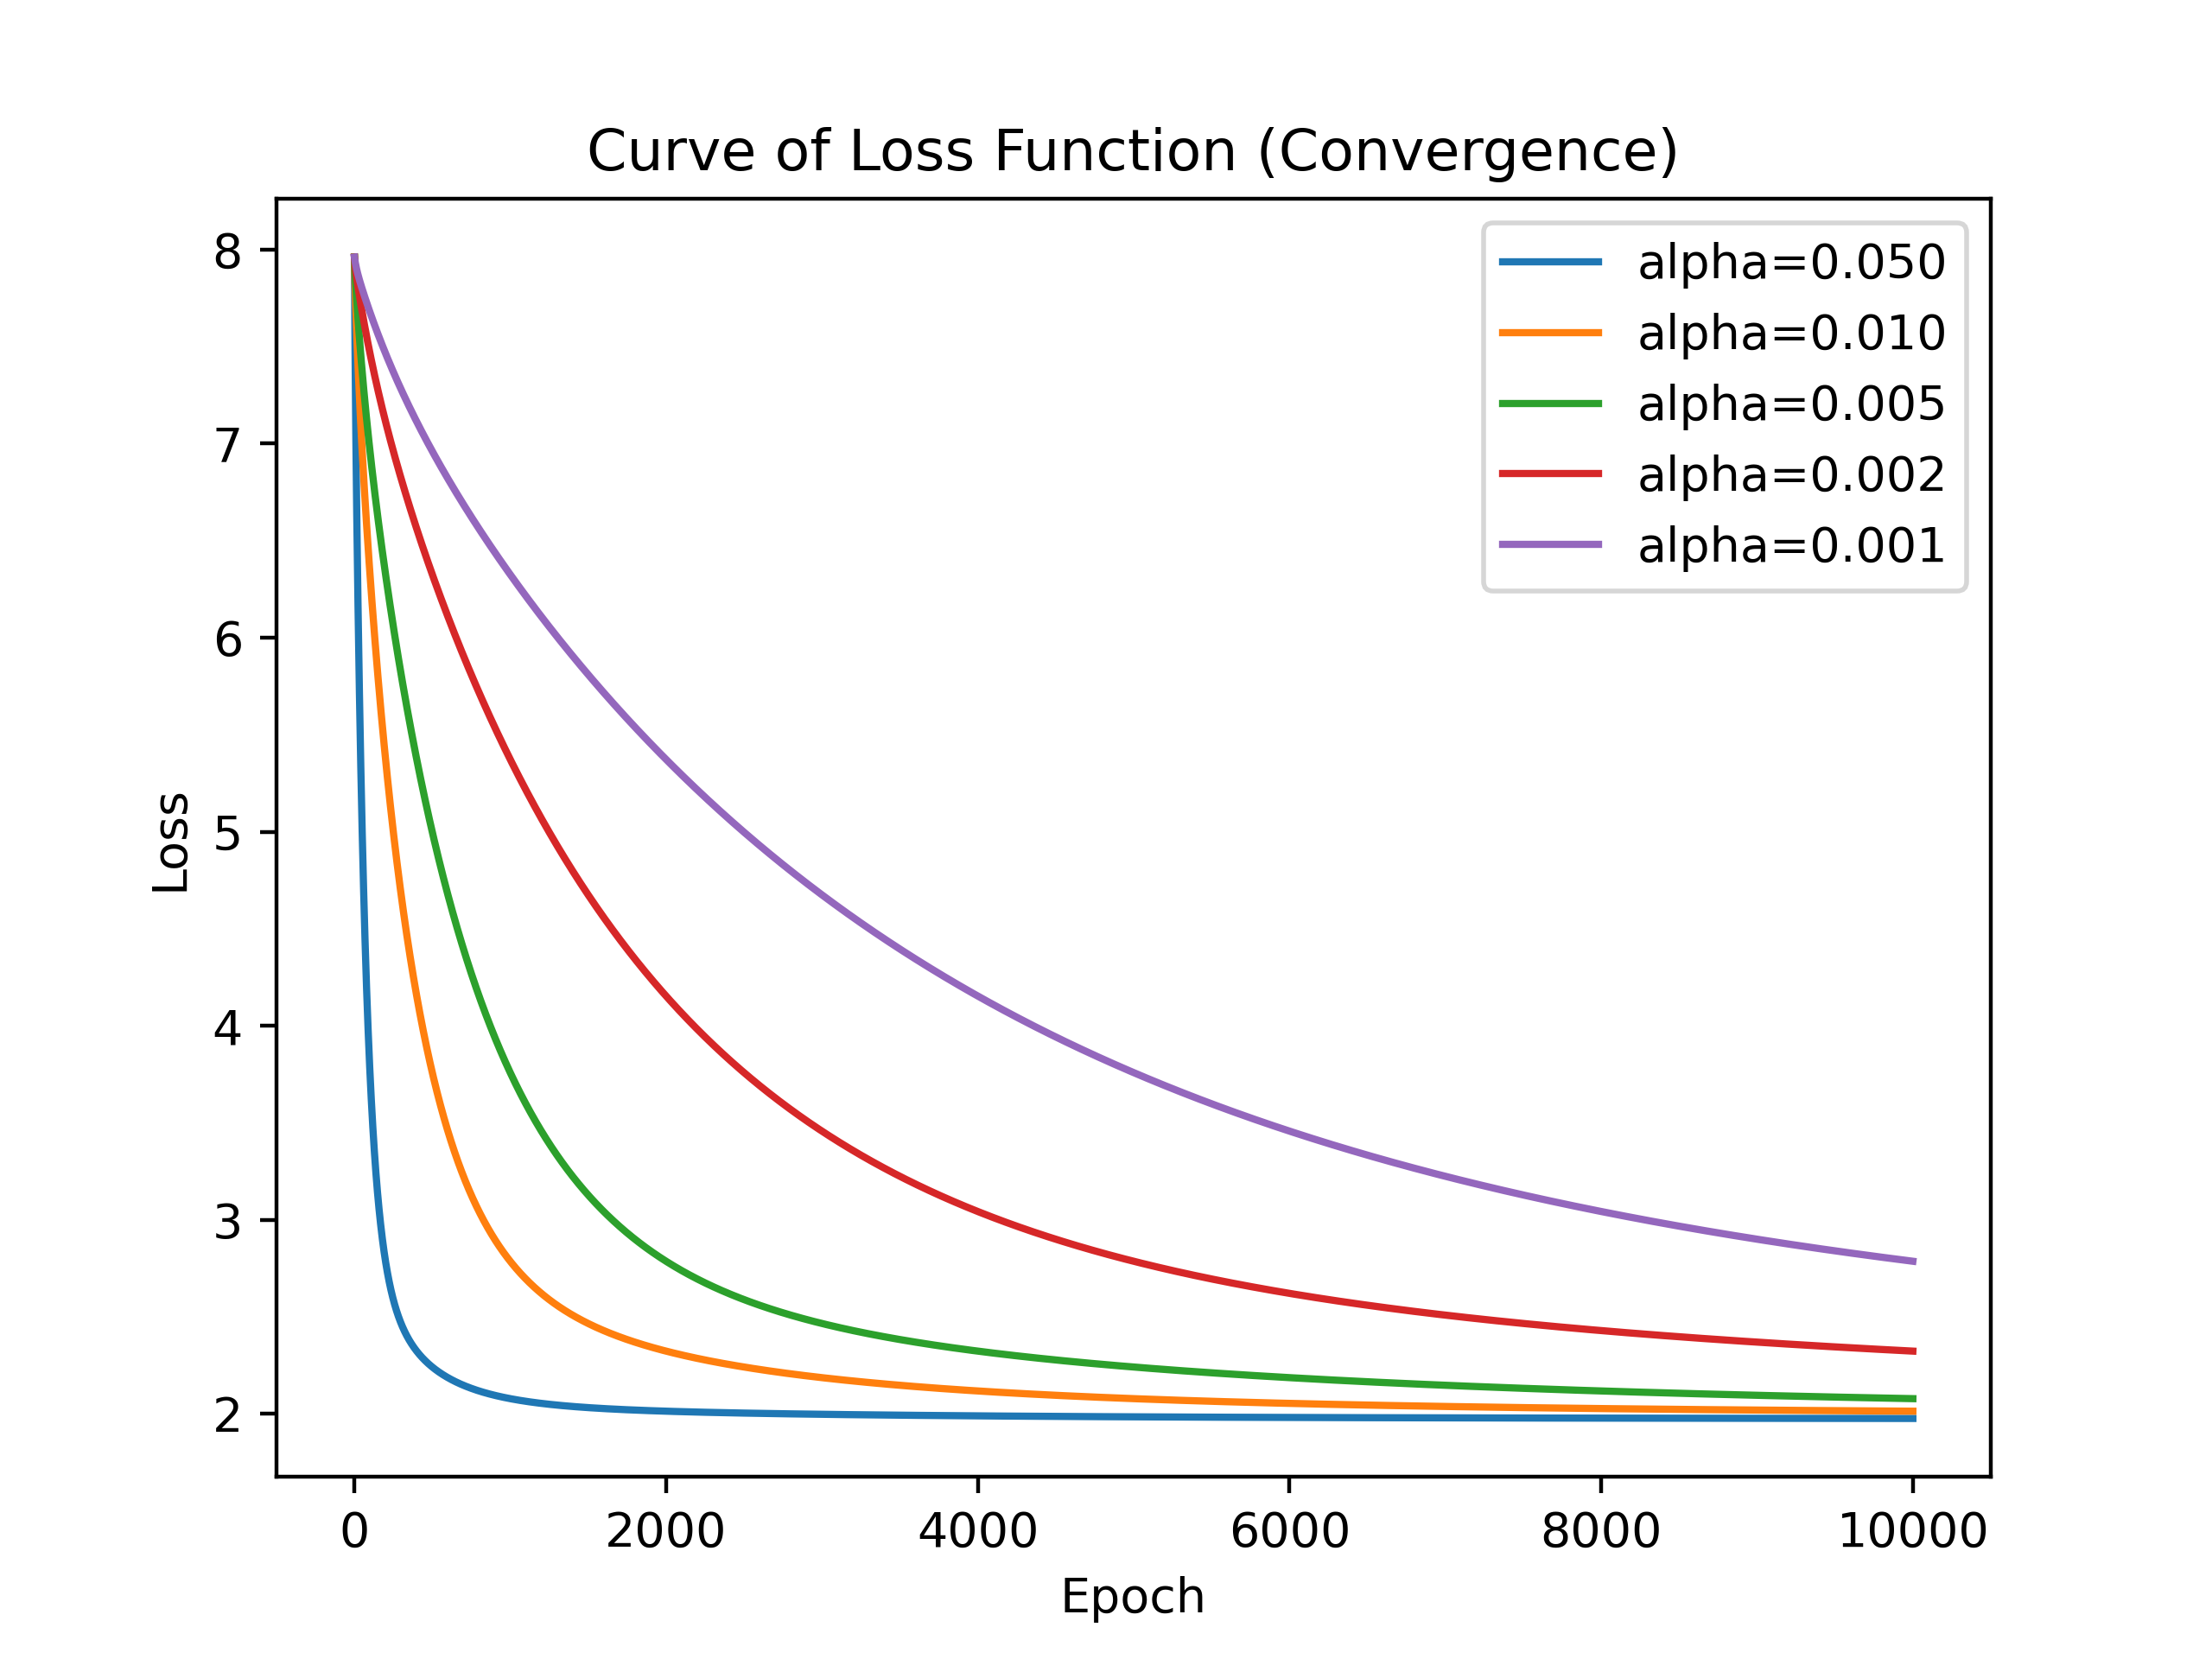
\includegraphics[width=0.84\textwidth]{./assets/SGD_lr_convergence.png}
        \caption{不同步长下训练集上的损失函数的变化曲线}
        \end{figure}

        \begin{figure}[htbp]
        \centering
        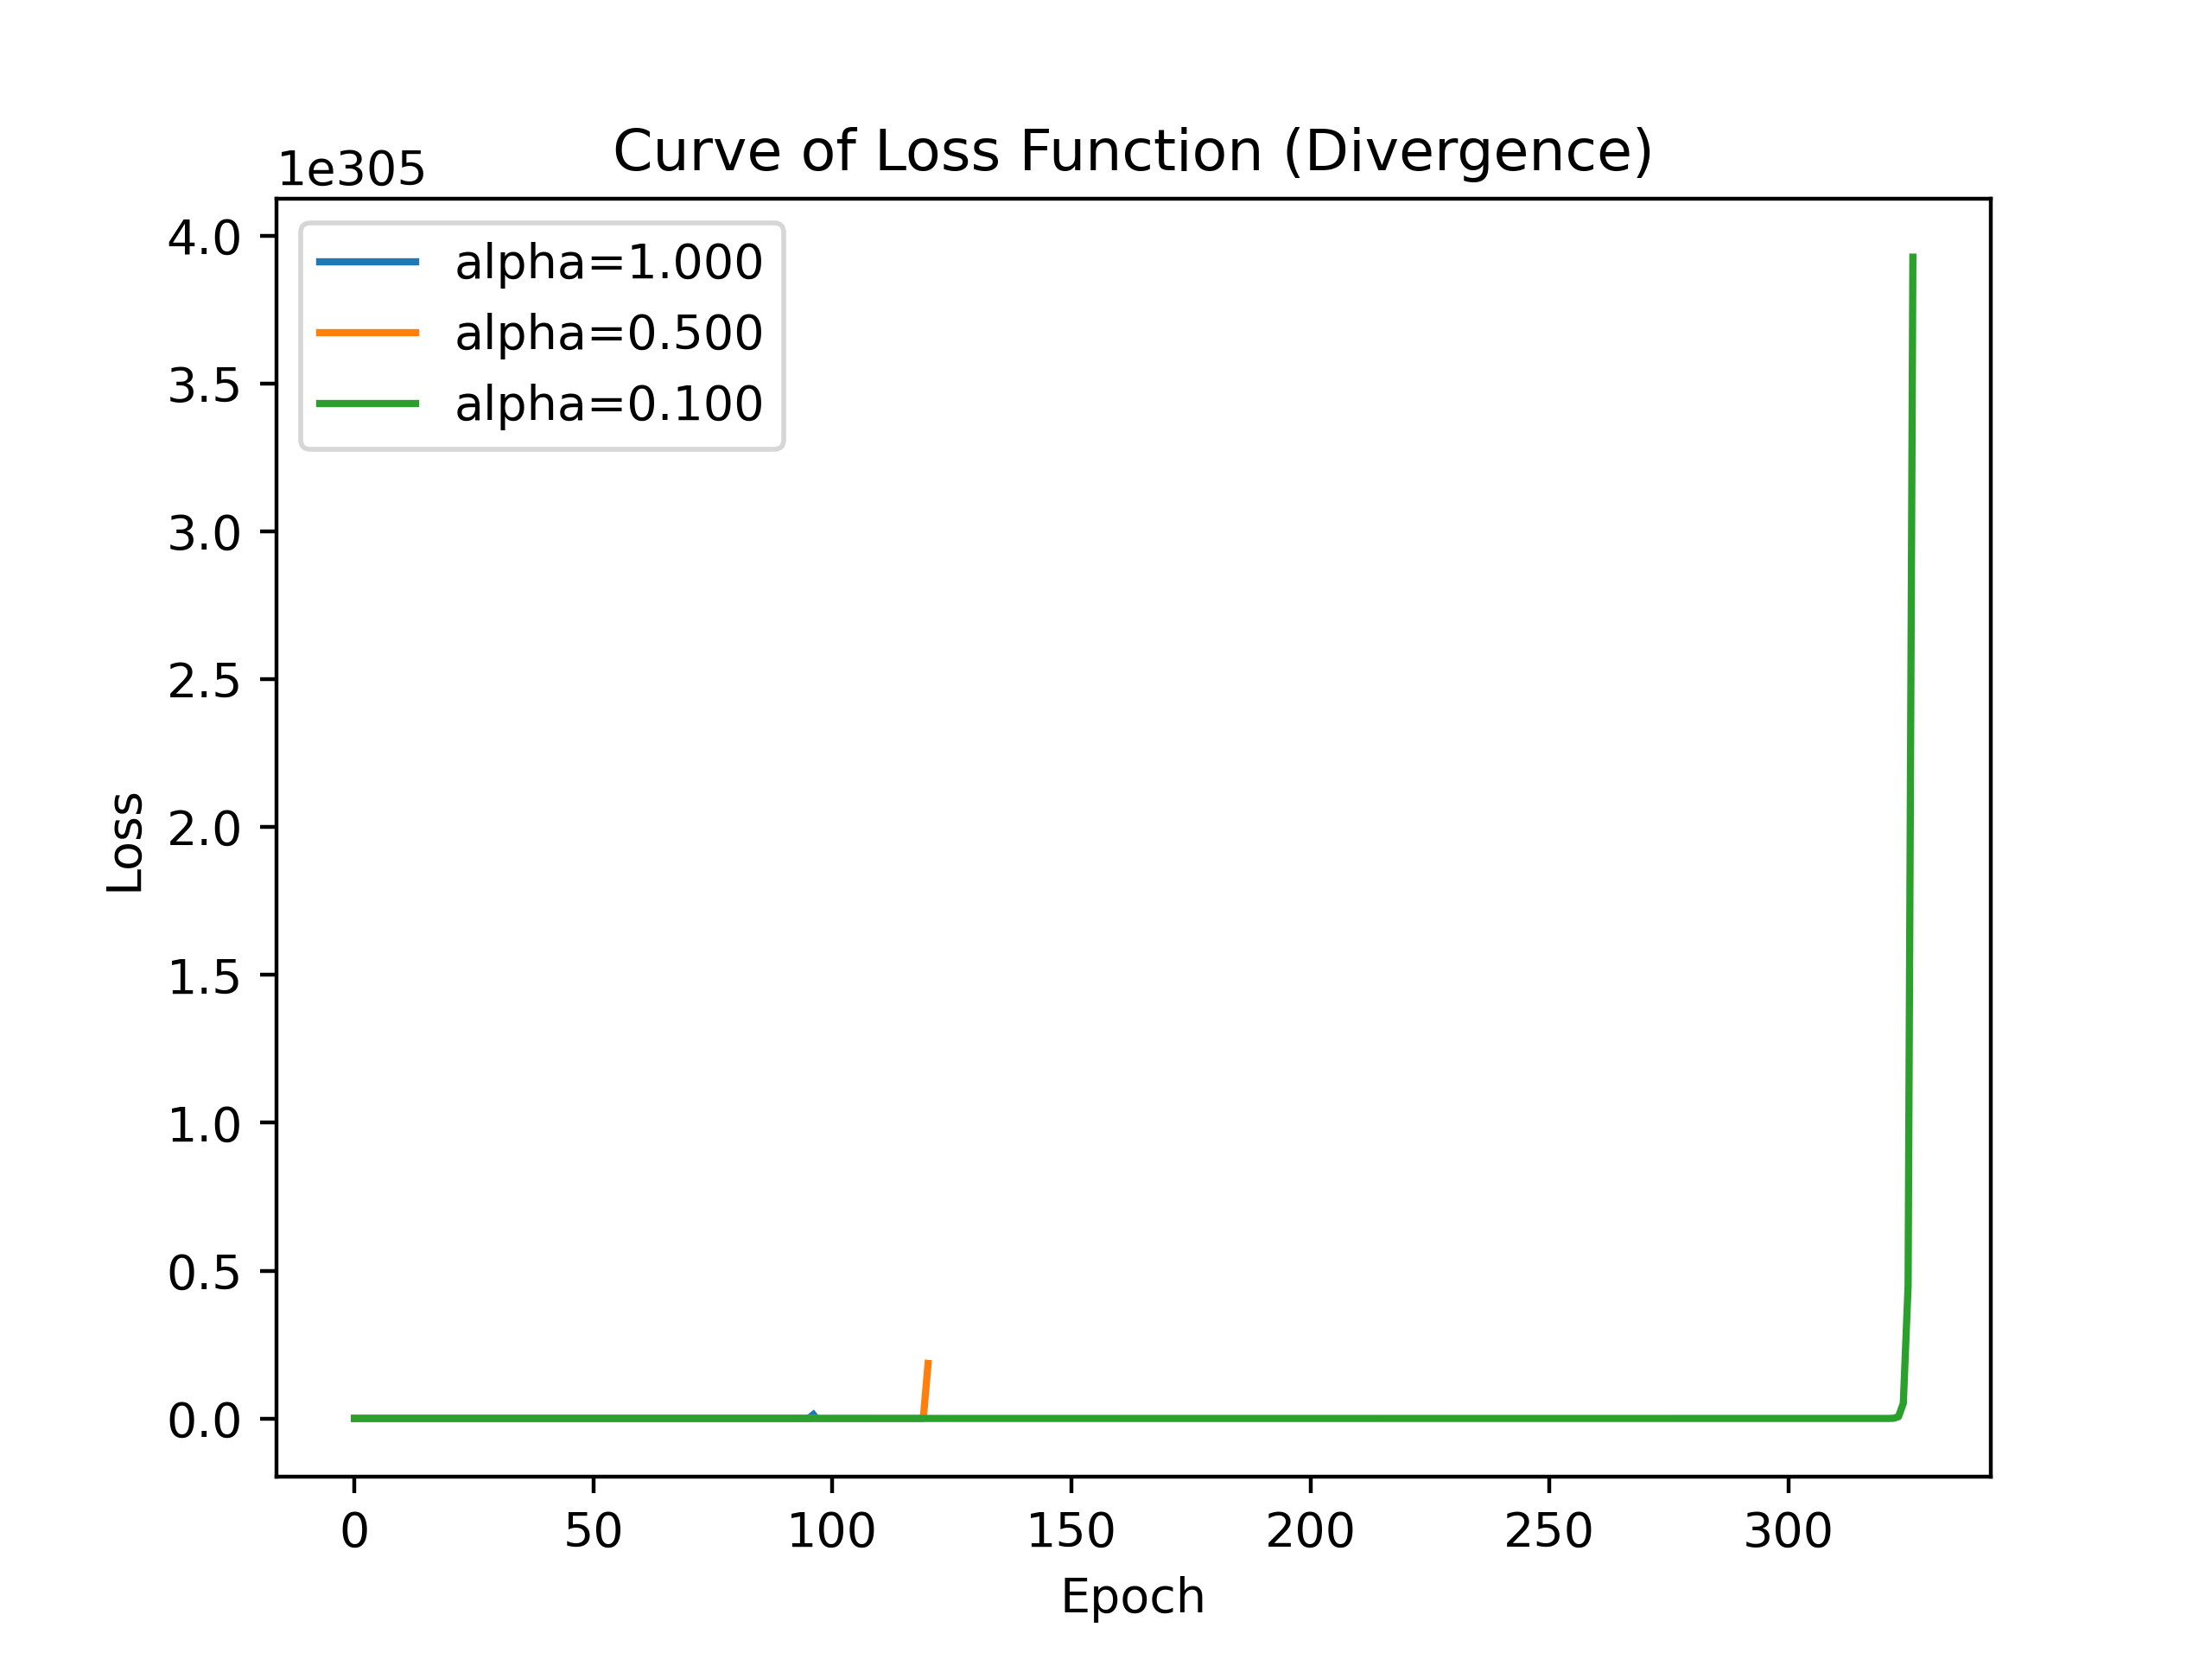
\includegraphics[width=0.84\textwidth]{./assets/SGD_lr_divergence.png}
        \caption{不同步长下训练集上的损失函数的变化曲线}
        \end{figure}

    \subsection{随机梯度下降}

    \subsubsection{SGD算法中梯度的表达式}

        对于自$\{1, 2, ..., m\}$中等概率地独立同分布采样得到的$q_1, q_2, ..., q_n$，
        我们定义抽样矩阵$\imat{S} = (s_{i j}) \in \mathbb{R}^{n \times m}$，
        满足$\forall i \in \{1, 2, ..., n\}$，$\forall j \in \{1, 2, ..., m\}$，有：
        $$
        s_{i j} =
        \begin{cases}
        0 & \text{if \quad} j \neq q_i  \\
        1 & \text{if \quad} j = q_i
        \end{cases}
        $$

        则随机梯度下降算法中的优化目标函数$J_{SGD}(\thetav)$可表示为：
        \begin{equation}\begin{aligned}
        J_{SGD}(\thetav) = \frac{1}{n} \Vert \imat{S} \Xm \thetav - \imat{S} \yv \Vert_2^2 + \lambda \thetav^T \thetav
        \end{aligned}\end{equation}

        因此，梯度$\nabla J_{SGD}(\thetav)$的表达式为：
        \begin{equation}\begin{aligned}
        \nabla J_{SGD}(\thetav) = \frac{2}{n} \Xm^T \imat{S}^T \imat{S}(\Xm \thetav - \yv) + 2 \lambda \thetav
        \end{aligned}\end{equation}

    \subsubsection{证明SGD算法下的梯度是对原梯度的无偏估计}

        命题$\mathbb{E}[\nabla J_{SGD}(\thetav)] = \nabla J(\thetav)$，等价于：
        \begin{align*}
        \mathbb{E}[\frac{2}{n} \Xm^T \imat{S}^T \imat{S} (\Xm \thetav - \yv) + 2 \lambda \thetav] = \frac{2}{m} \Xm^T (\Xm \thetav - \yv) + 2 \lambda \thetav
        \end{align*}

        由于期望的线性性质，我们有：
        \begin{align*}
        \mathbb{E}[\frac{2}{n} \Xm^T \imat{S}^T \imat{S} (\Xm \thetav - \yv) + 2 \lambda \thetav]
        = \frac{2}{n} \Xm^T \mathbb{E}[\imat{S}^T \imat{S}] (\Xm \thetav - \yv) + 2 \lambda \thetav
        \end{align*}

        对比两式，我们只需证明：
        \begin{align*}
        \mathbb{E}[\imat{S}^T \imat{S}] = \frac{n}{m} \imat{I}_m
        \end{align*}

        $\imat{S}^T \imat{S} \in \mathbb{R}^{m \times m}$。
        对$\forall k, p \in \{1, 2, ..., m\}$，设$\imat{S}^T \imat{S}$的第$k$行第$p$列元素为$r_{kp}$，计算易得：
        \begin{align*}
        r_{kp} = \sum_{u = 1}^{n} s_{uk}s_{up}
        \end{align*}

        考虑$\imat{S}$的定义，当$j$固定时，$s_{uj} = 1$当且仅当$j = q_u$，否则等于0。
        因此，若$k \ne p$，则$k$、$p$至少有一个不等于$q_u$，于是：
        \begin{align*}
        r_{kp} = \sum_{u = 1}^{n} s_{uk}s_{up} = \sum_{u = 1}^{n} 0 = 0
        \end{align*}

        若$k = p = j$，由于$q_u$等概率地取$\{1, 2, ..., m\}$中的一个值。
        因此$s_{uj}$是一个随机变量，有$\frac{1}{m}$的概率等于1，否则于0，此时有：
        \begin{align*}
        \mathbb{E}[r_{kp}] = \sum_{u = 1}^{n} \mathbb{E}[s_{uj}^2] = \sum_{u = 1}^{n} \frac{1}{m} = \frac{n}{m}
        \end{align*}

        综上，我们证明了$\mathbb{E}[\imat{S}^T \imat{S}] = \frac{n}{m} \imat{I}_m$成立。

        原命题成立，证毕。

    \subsubsection{SGD算法的实现}

        参见./SGD/startcode.py文件中的stochastic\_grad\_descent函数。

    \subsubsection{batch\_size调整}

        固定$\lambda = 0$，固定步长$\eta = 0.005$，调整batch\_size的值，观察梯度下降算法的收敛情况。
        在训练集上的损失函数的变化曲线如图3所示，在验证集上的损失函数的变化曲线如图4所示。

        我们测试了batch\_size为1、2、4、8、16、32、64和128的情况。
        从图中可以看出，不同的batch\_size下，算法的收敛速度几乎一致。
        但是，随着batch\_size的增大，算法的收敛过程逐渐变得更平滑，波动幅度也逐渐减小。
        因此，我们认为batch\_size越大，算法的收敛也就越稳定。

        \begin{figure}[htbp]
        \centering
        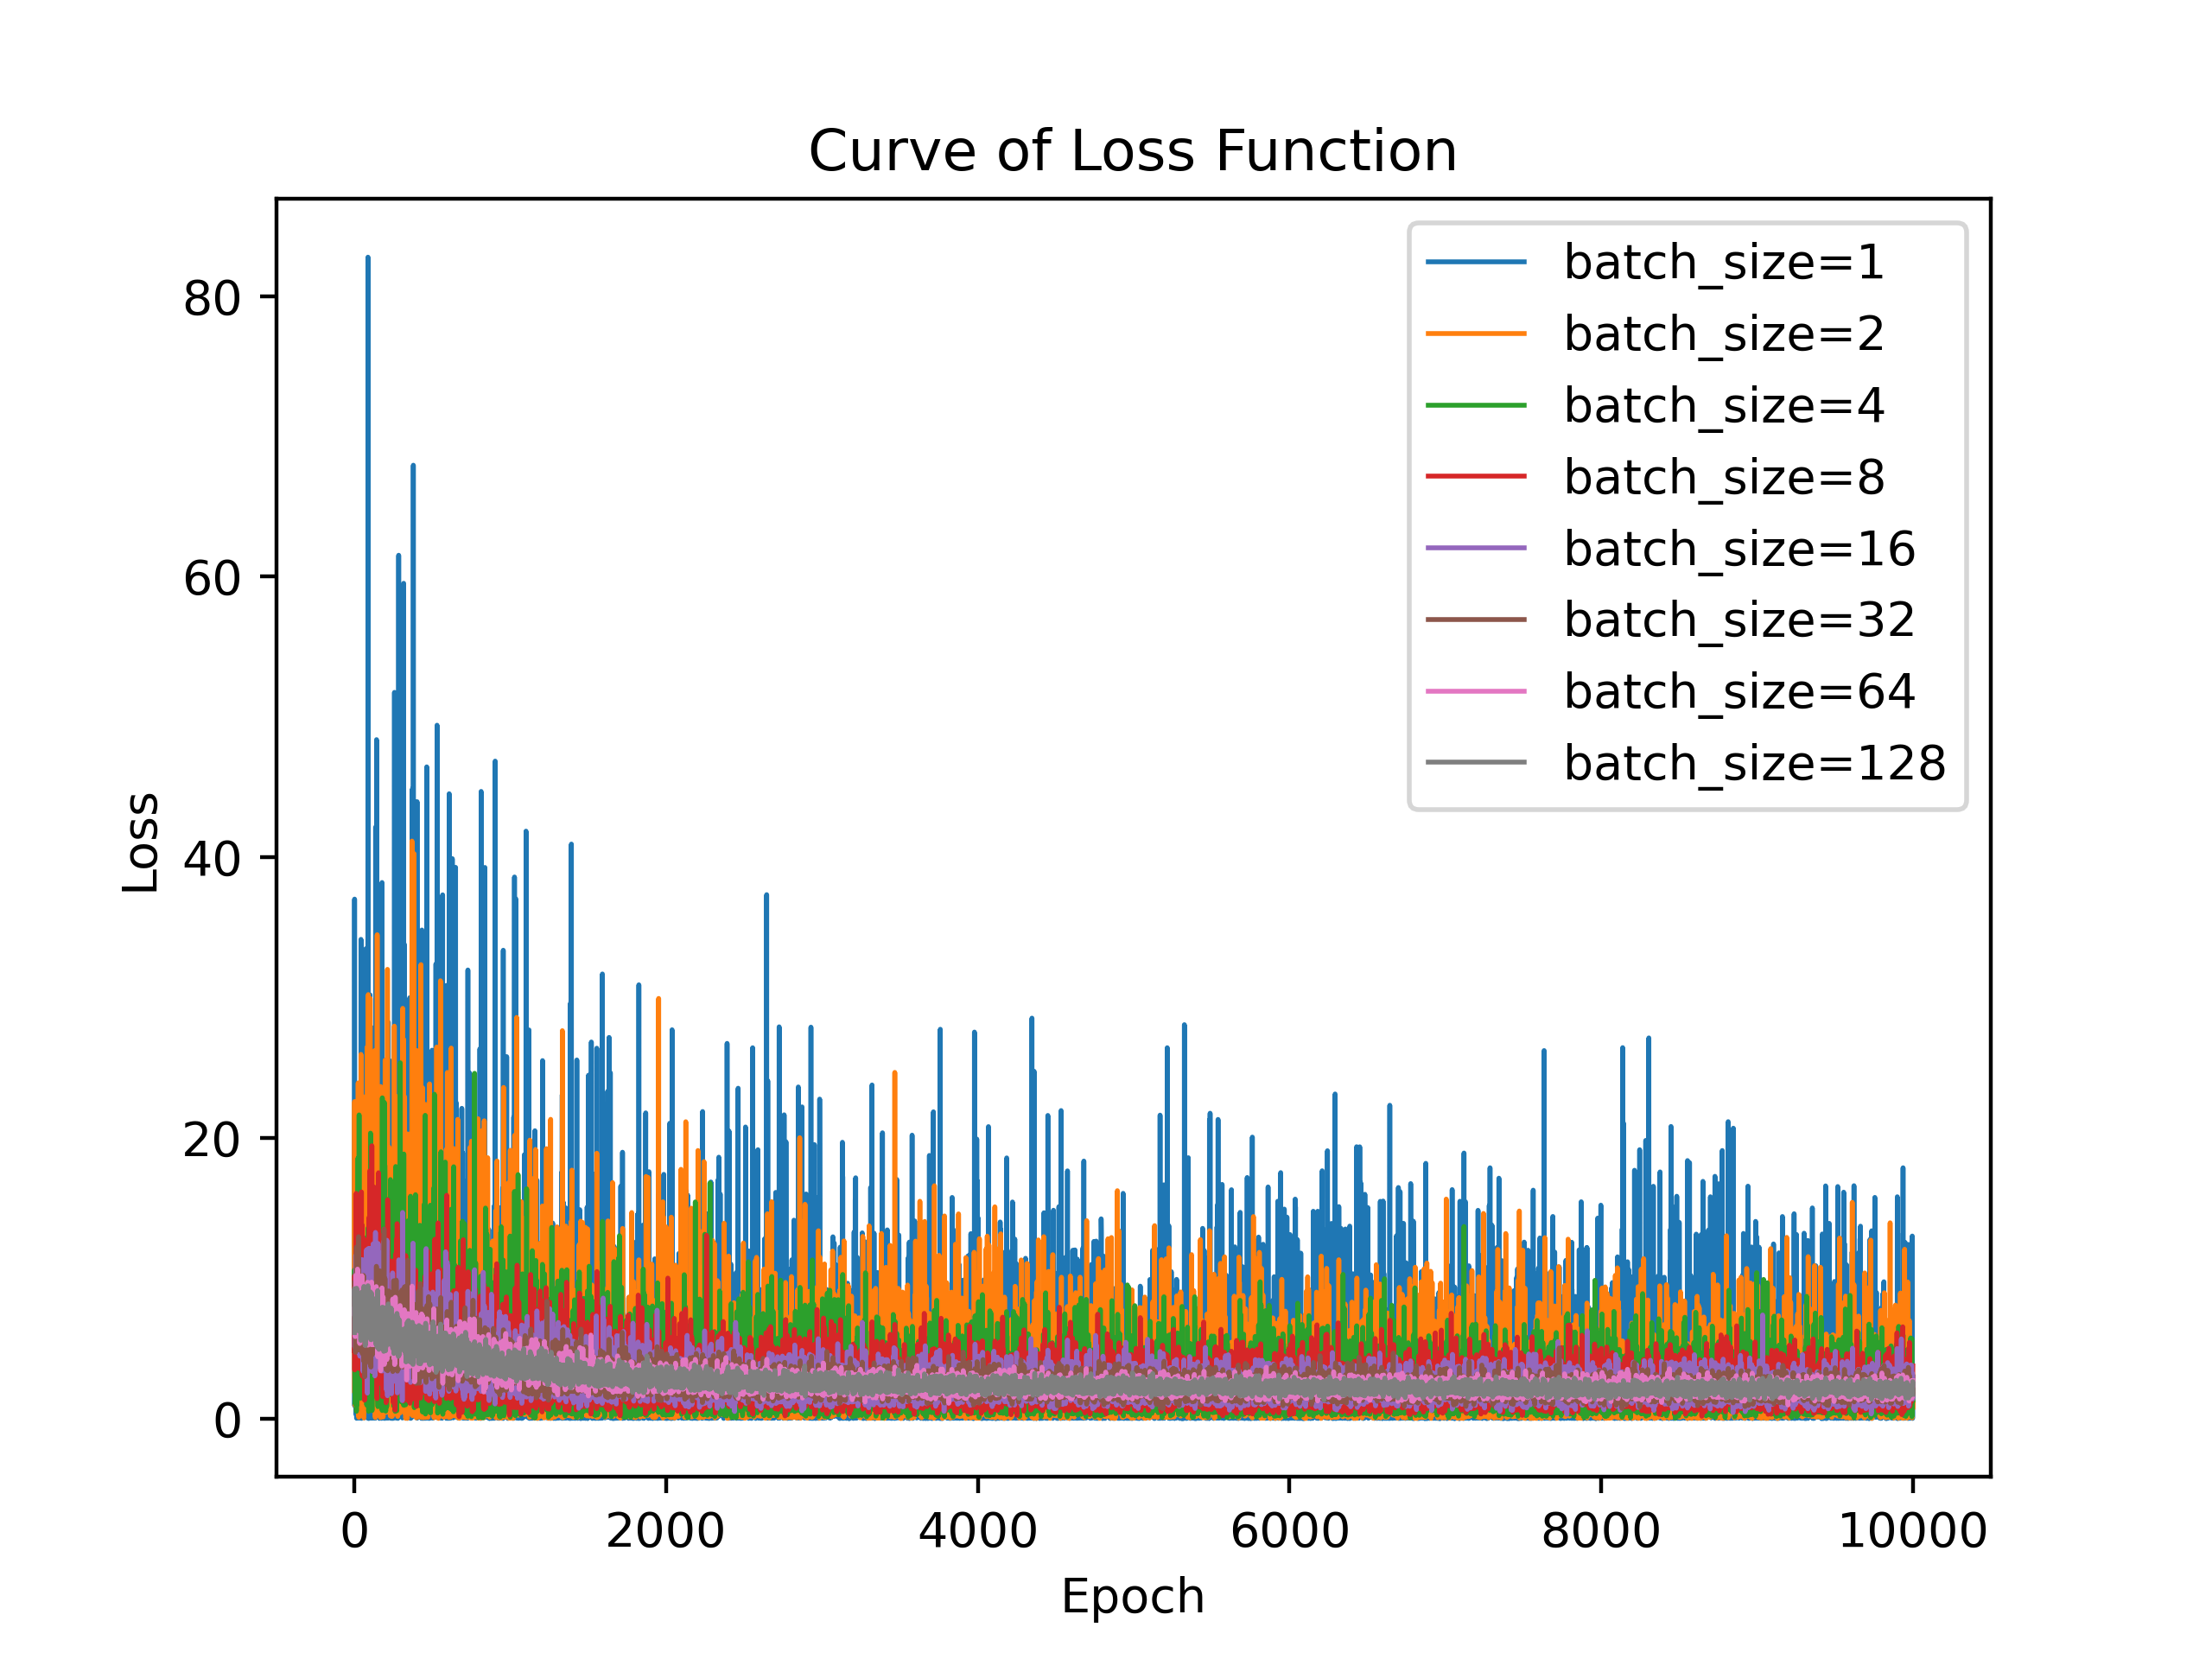
\includegraphics[width=0.84\textwidth]{./assets/SGD_batch_train.png}
        \caption{不同批大小下训练集上的损失函数的变化曲线}
        \end{figure}

        \begin{figure}[htbp]
        \centering
        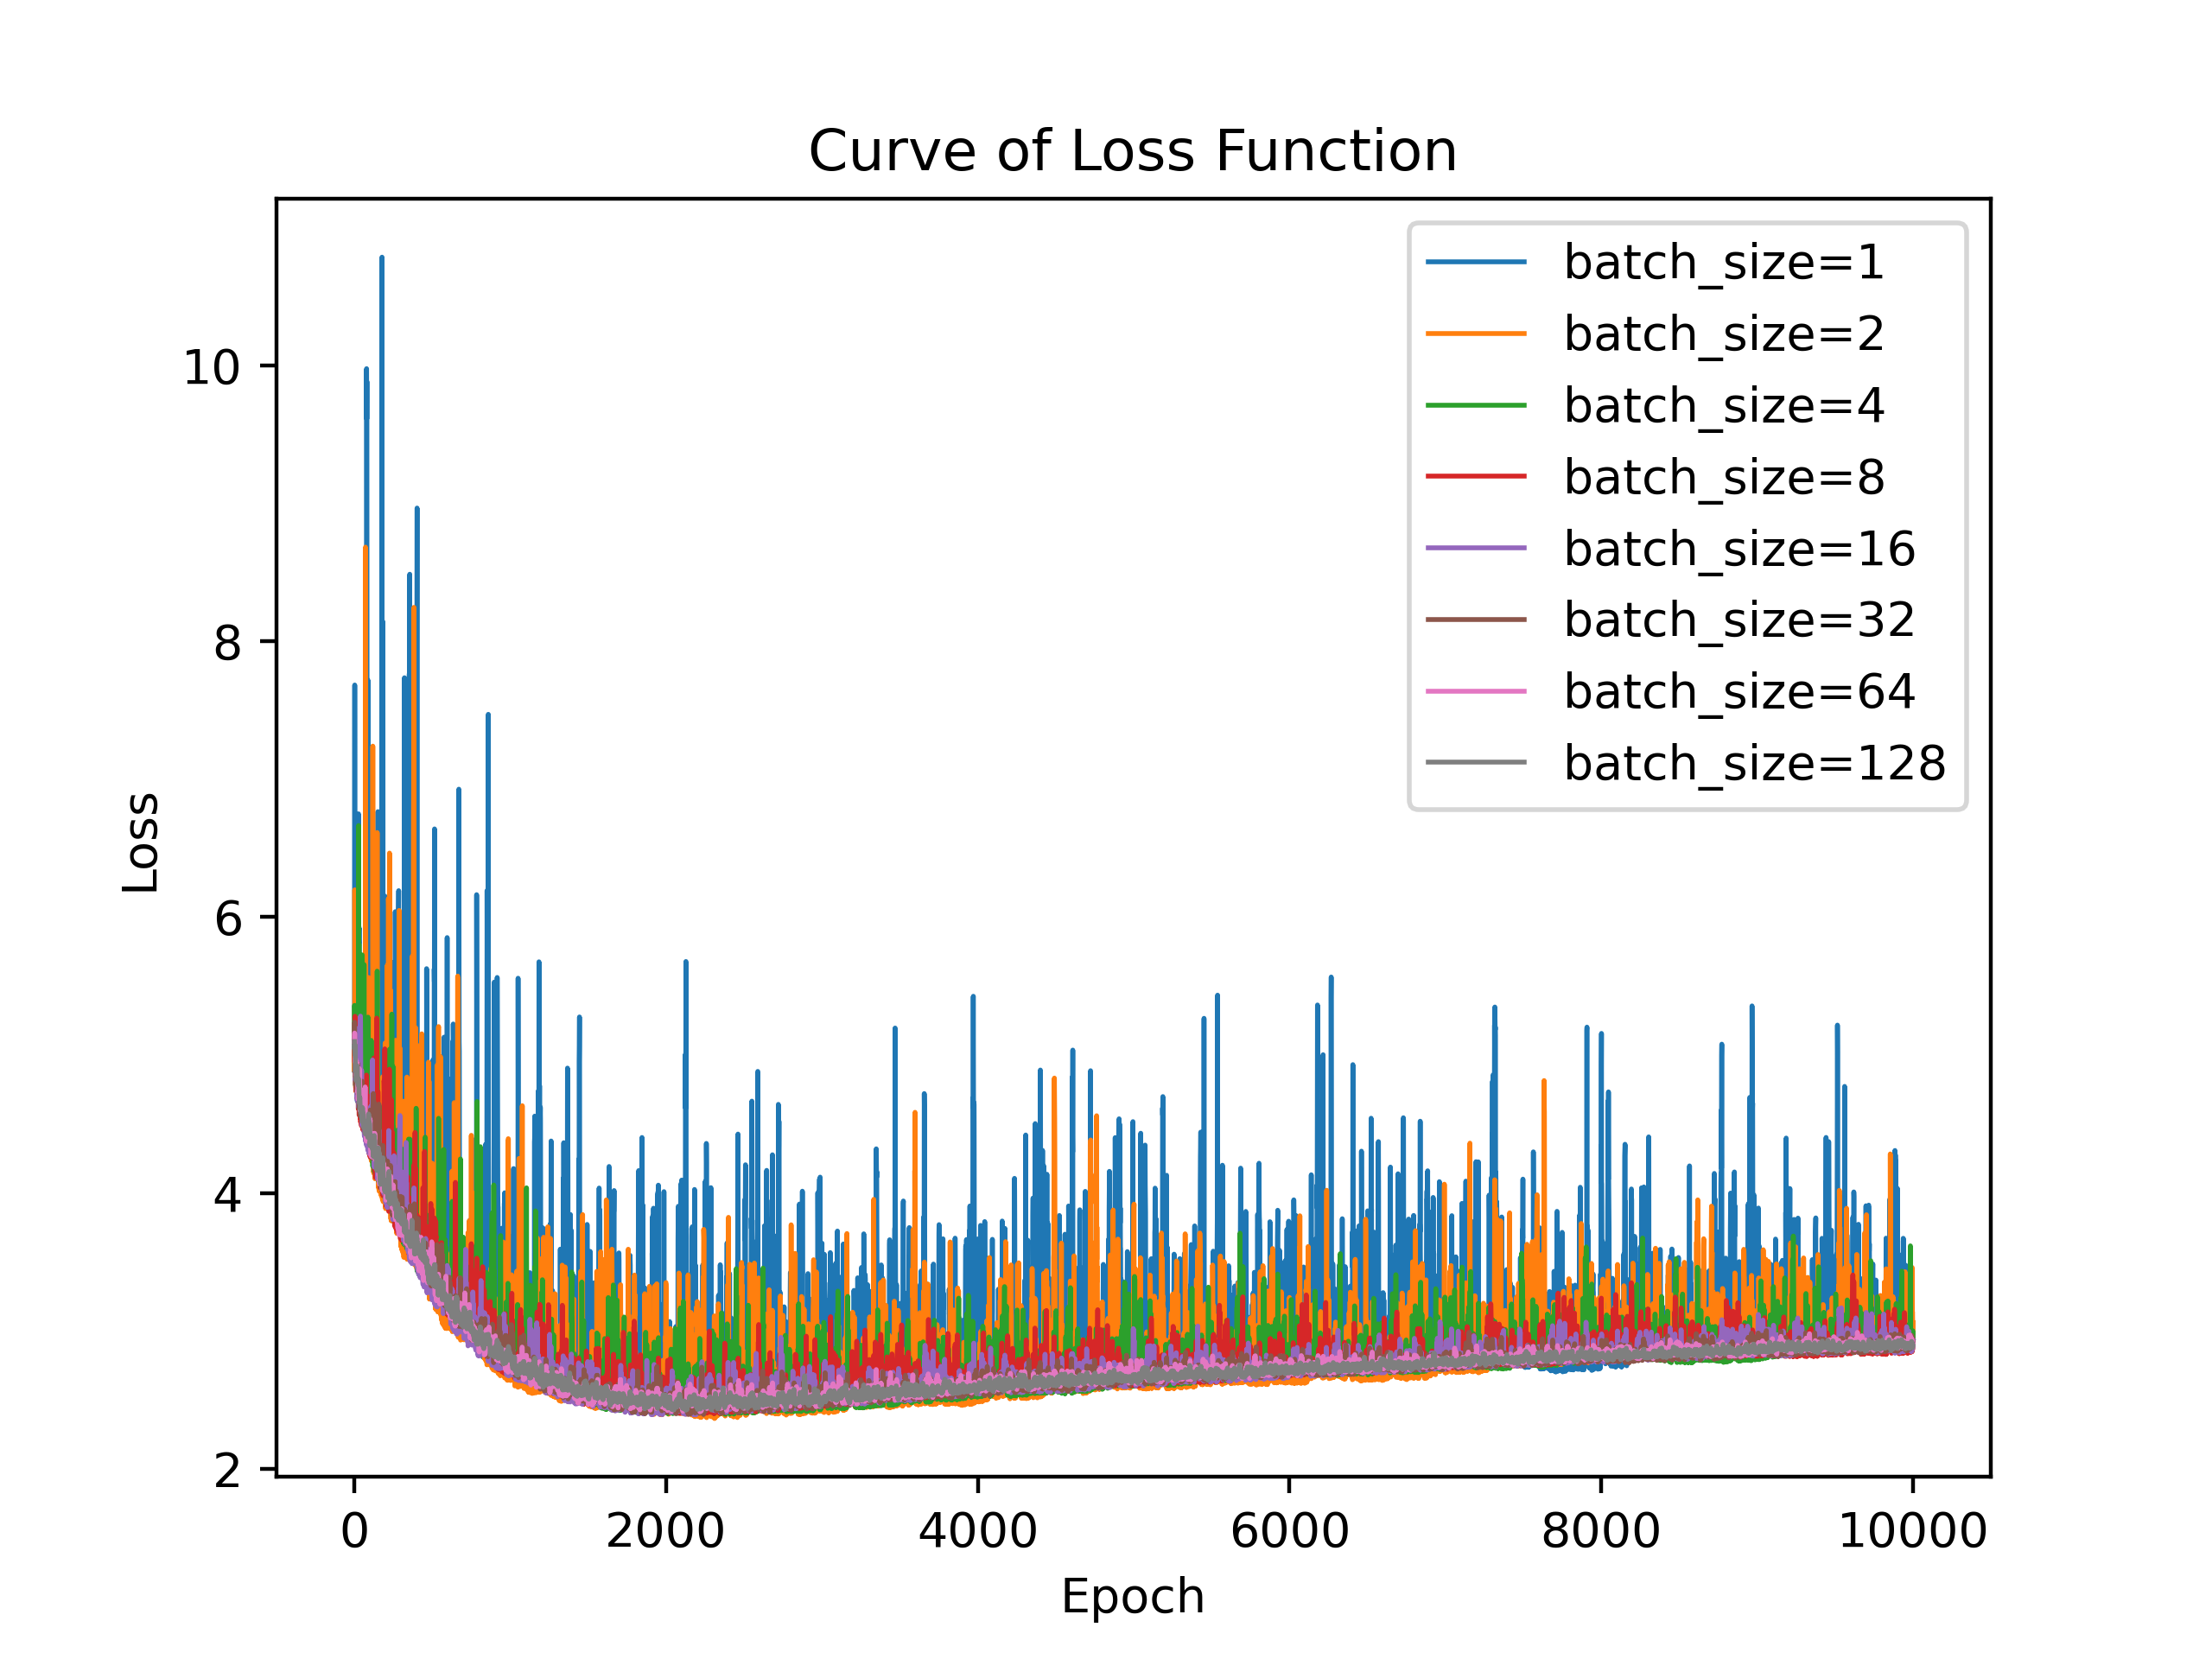
\includegraphics[width=0.84\textwidth]{./assets/SGD_batch_valid.png}
        \caption{不同批大小下验证集上的损失函数的变化曲线}
        \end{figure}

        在batch\_size=128，初始步长为0.01时，我们取不同的步长调整策略，观察梯度下降算法的收敛情况。
        在训练集上的损失函数的变化曲线如图5所示，在验证集上的损失函数的变化曲线如图6所示。

        \begin{figure}[htbp]
        \centering
        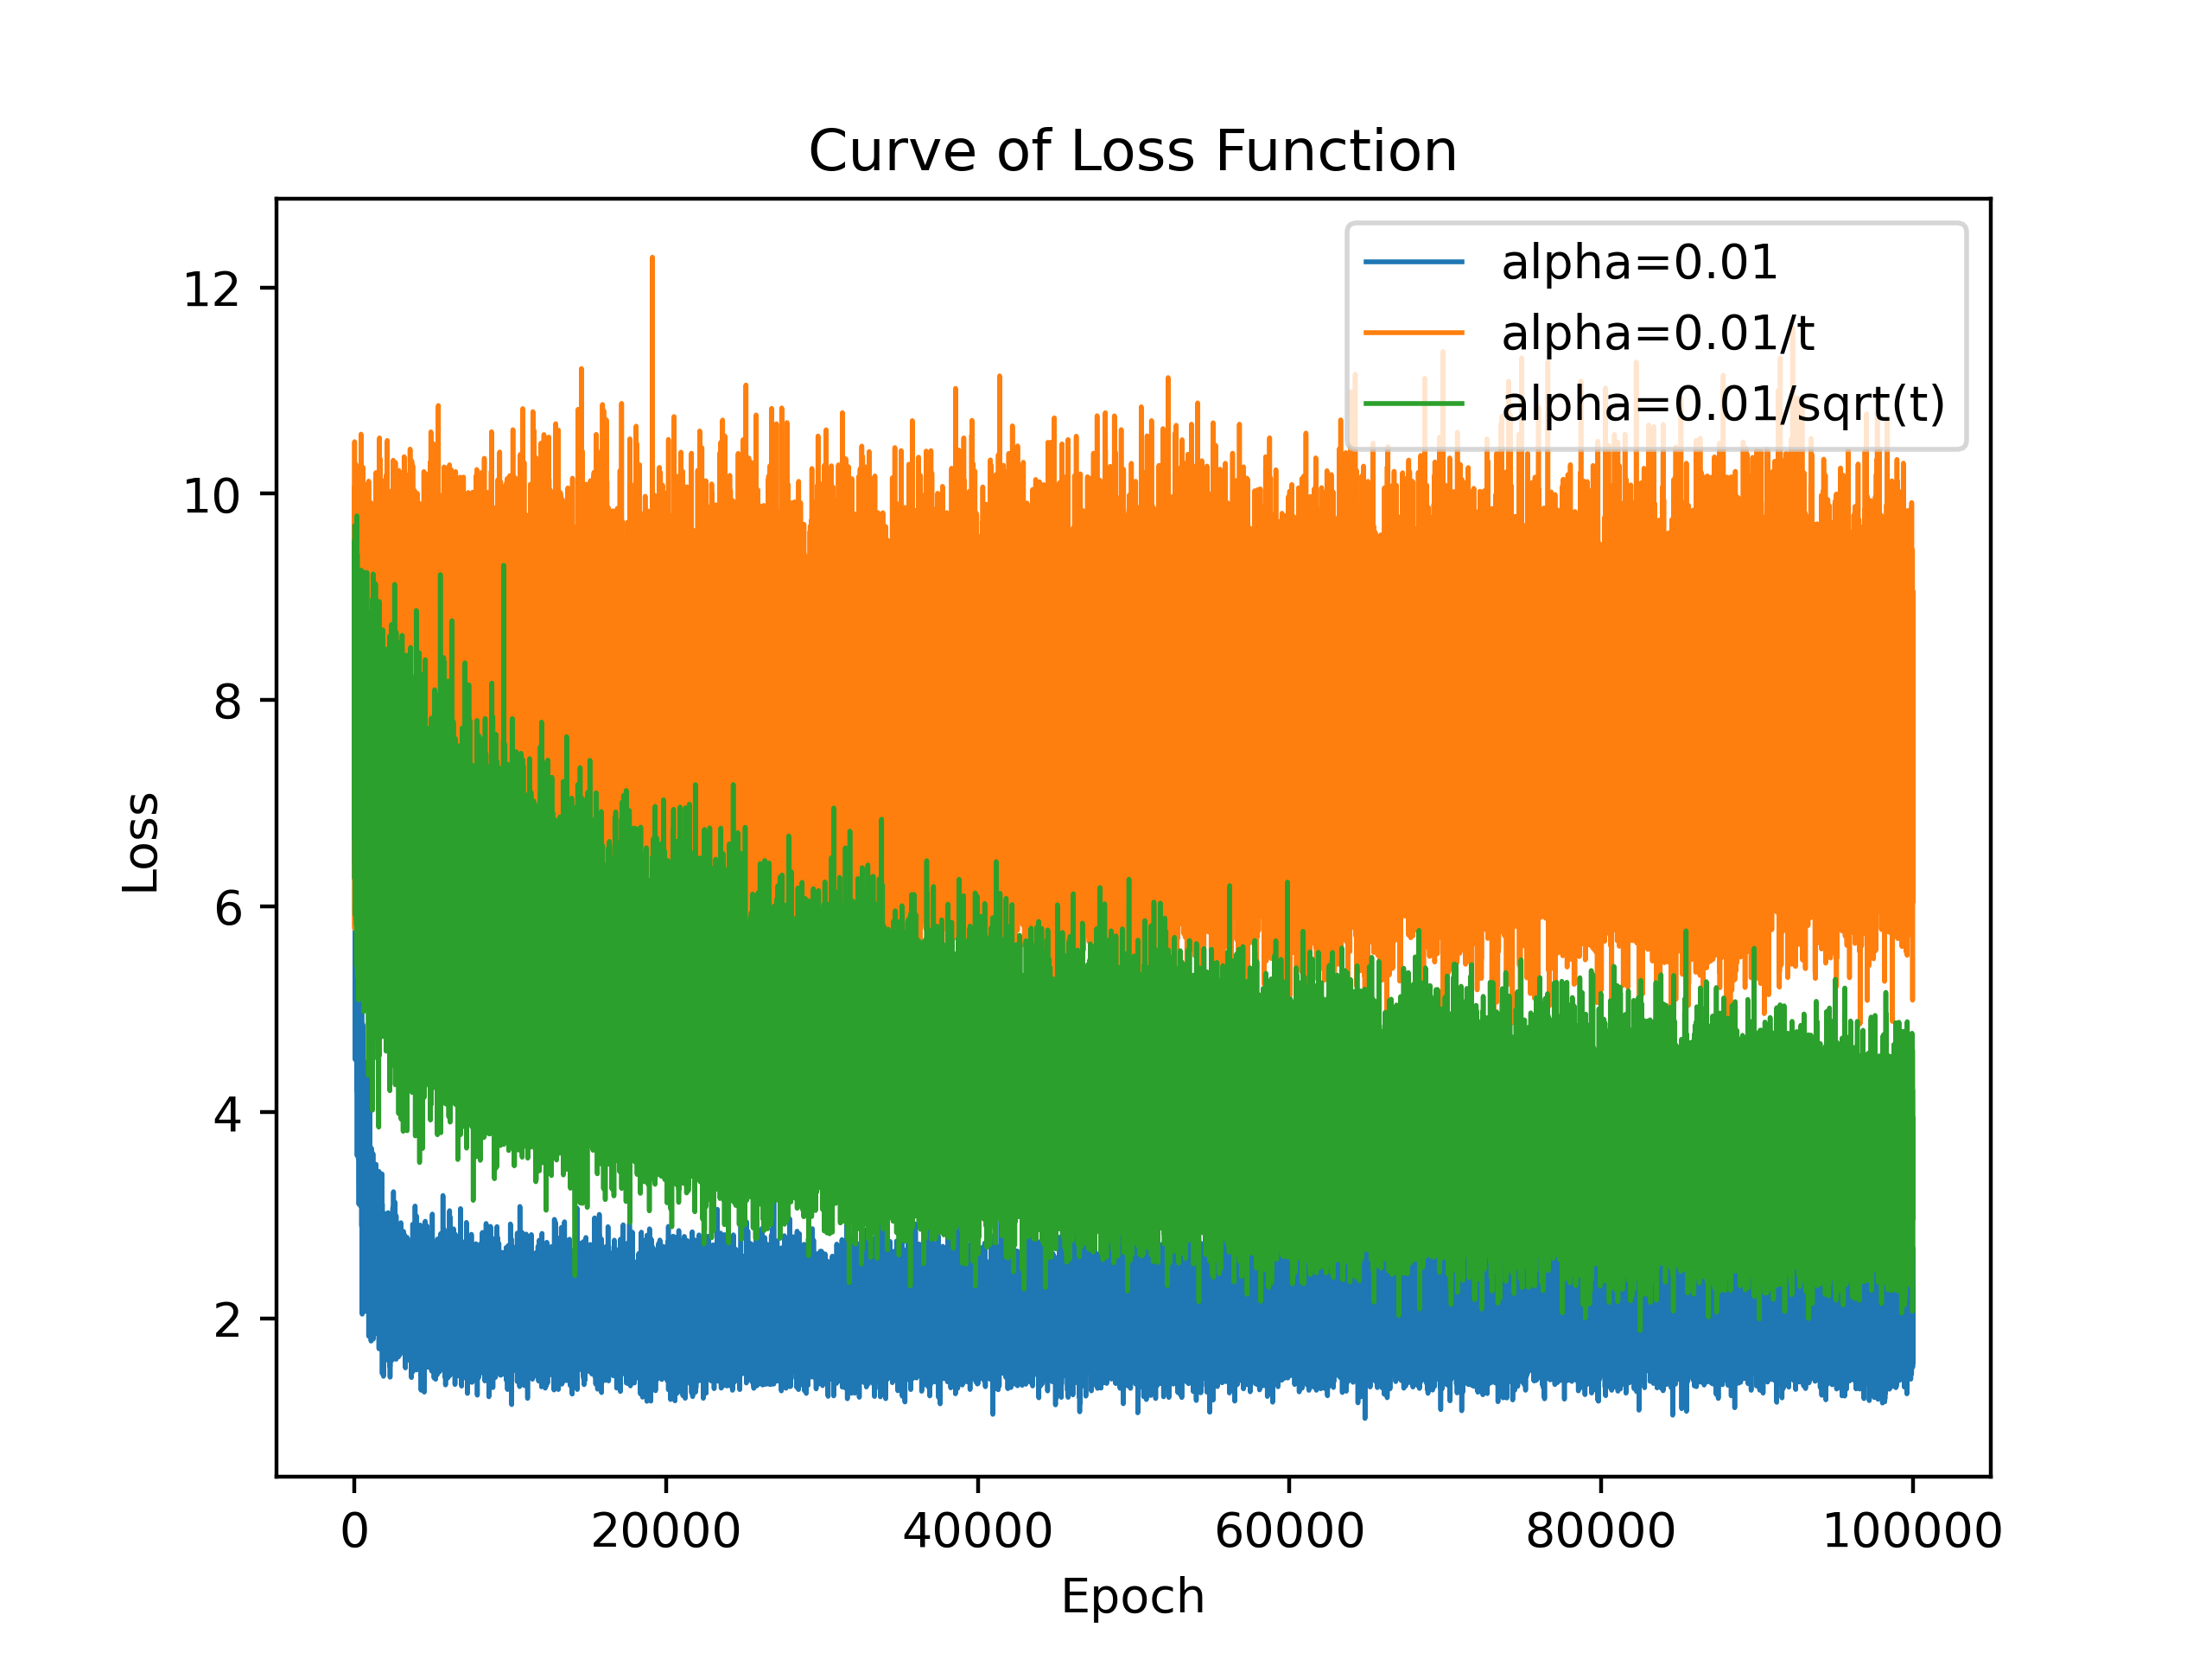
\includegraphics[width=0.84\textwidth]{./assets/SGD_lr_strategies_train.png}
        \caption{不同步长调整策略下训练集上的损失函数的变化曲线}
        \end{figure}

        \begin{figure}[htbp]
        \centering
        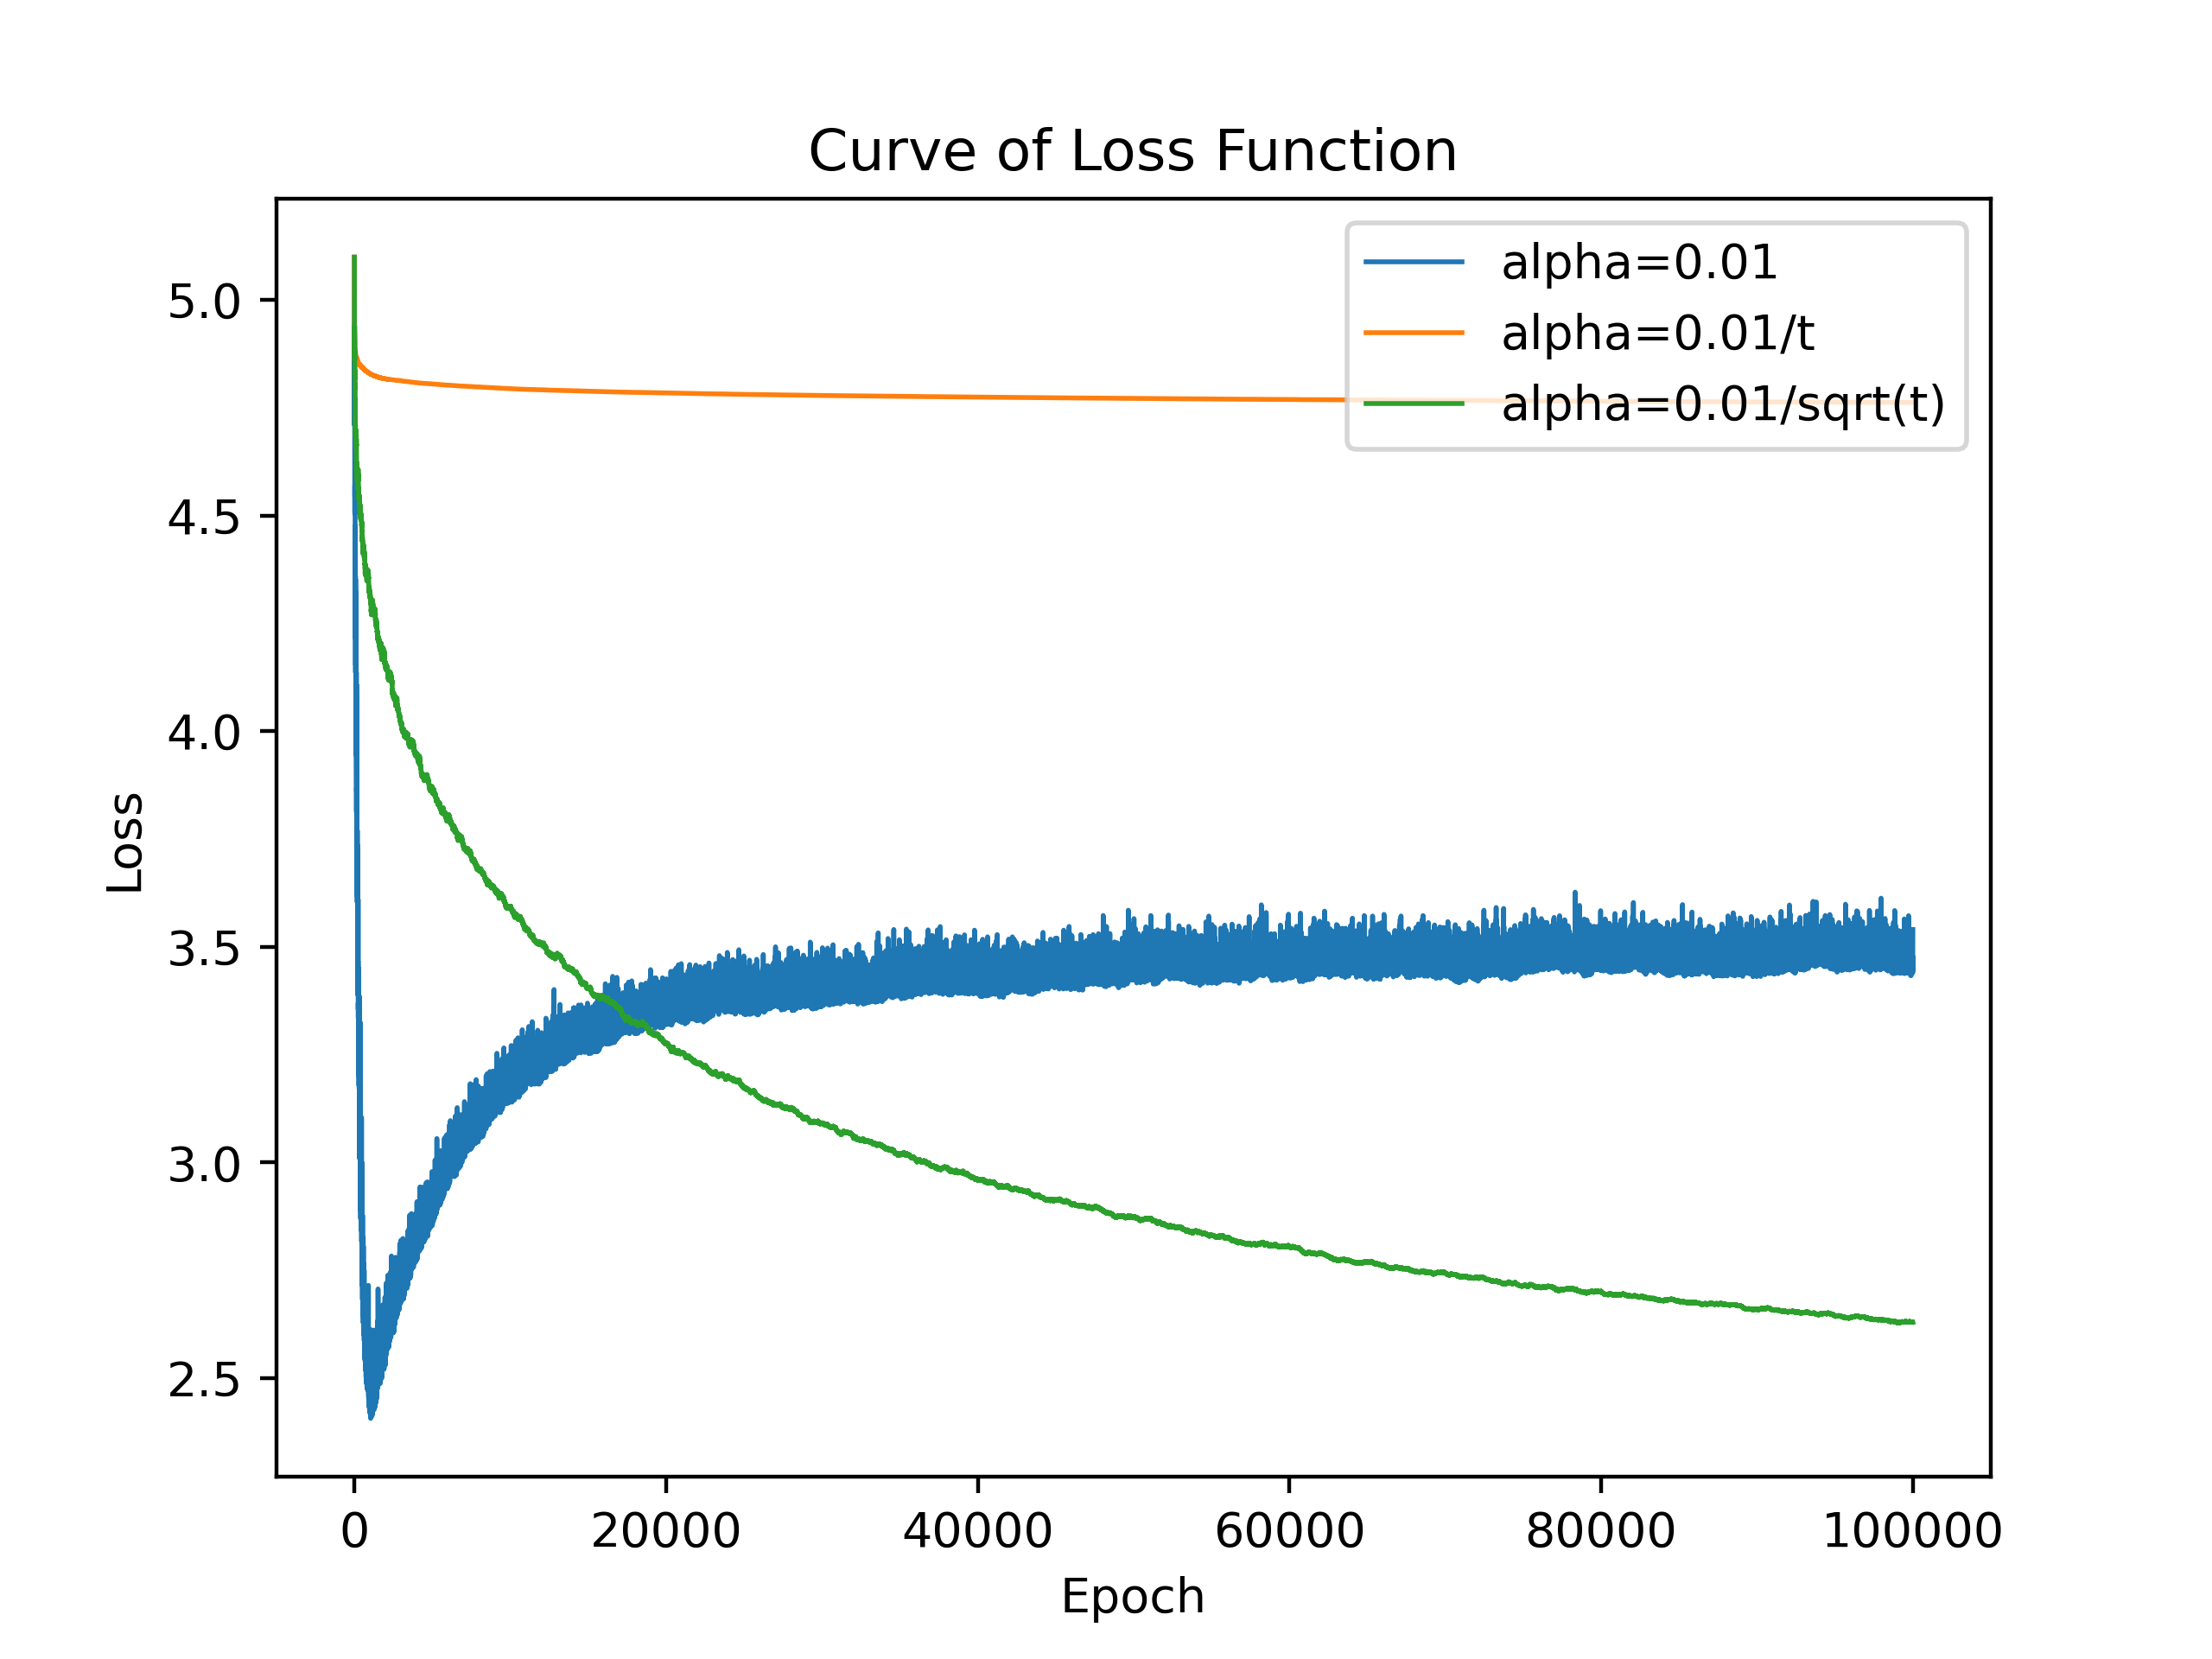
\includegraphics[width=0.84\textwidth]{./assets/SGD_lr_strategies_valid.png}
        \caption{不同步长调整策略下验证集上的损失函数的变化曲线}
        \end{figure}

        可以看出，若取步长固定，算法的收敛速度较快，在训练集上的表现较为稳定，
        但在验证集上并不能收敛到最优参数位置，在后期甚至倾向于发散；
        若取步长随迭代次数呈反比例变化，算法在验证集上的收敛过程变得非常光滑，
        但此时算法在后期的收敛速度过慢，导致不能够收敛到最优参数位置；
        而若取步长随迭代次数的平方根呈反比例变化，我们发现算法的性能良好，
        在训练集上能够以合适的速度和稳定性收敛，在验证集上也能够光滑、快速地收敛到最优的参数位置。

        \textbf{综上，取batch\_size=128，步长调整策略为随迭代次数的平方根呈反比例变化，SGD算法的性能较好。}

    \subsection{模型选择}

    使用SGD算法，取batch\_size=128，初始步长为0.01，步长调整策略为随迭代次数的平方根呈反比例变化，迭代次数为100000次。

    我们取正则化系数$\lambda \in \{10^{-8}, 10^{-7}, ..., 10^{2}\}$，训练过程中模型在验证集上的损失函数值如图8所示，
    模型在验证集上的均方误差如表1所示。

    \begin{table}[htbp]
    \caption{在不同的正则化系数下，模型在验证集上的均方误差}
    \centering
    \begin{tabular}{cc}
        \toprule
        lambda         & MSE (valid)                \\
        \midrule
        $10^{-8}$      & 2.629872330826207          \\
        $10^{-7}$      & 2.630012511937801          \\
        $10^{-6}$      & 2.629049094324194          \\
        $\bm{10^{-5}}$ & \textbf{2.628083233220087} \\
        $10^{-4}$      & 2.629858879741408          \\
        $10^{-3}$      & 2.631048055957441          \\
        $10^{-2}$      & 2.673634035806118          \\
        $10^{-1}$      & 3.124097256730932          \\
        $10^0$         & 4.429540373987043          \\
        $10^1$         & 4.909692882584656          \\
        $10^2$         & 5.061860288433802
    \end{tabular}
    \end{table}

    \begin{figure}[htbp]
    \centering
    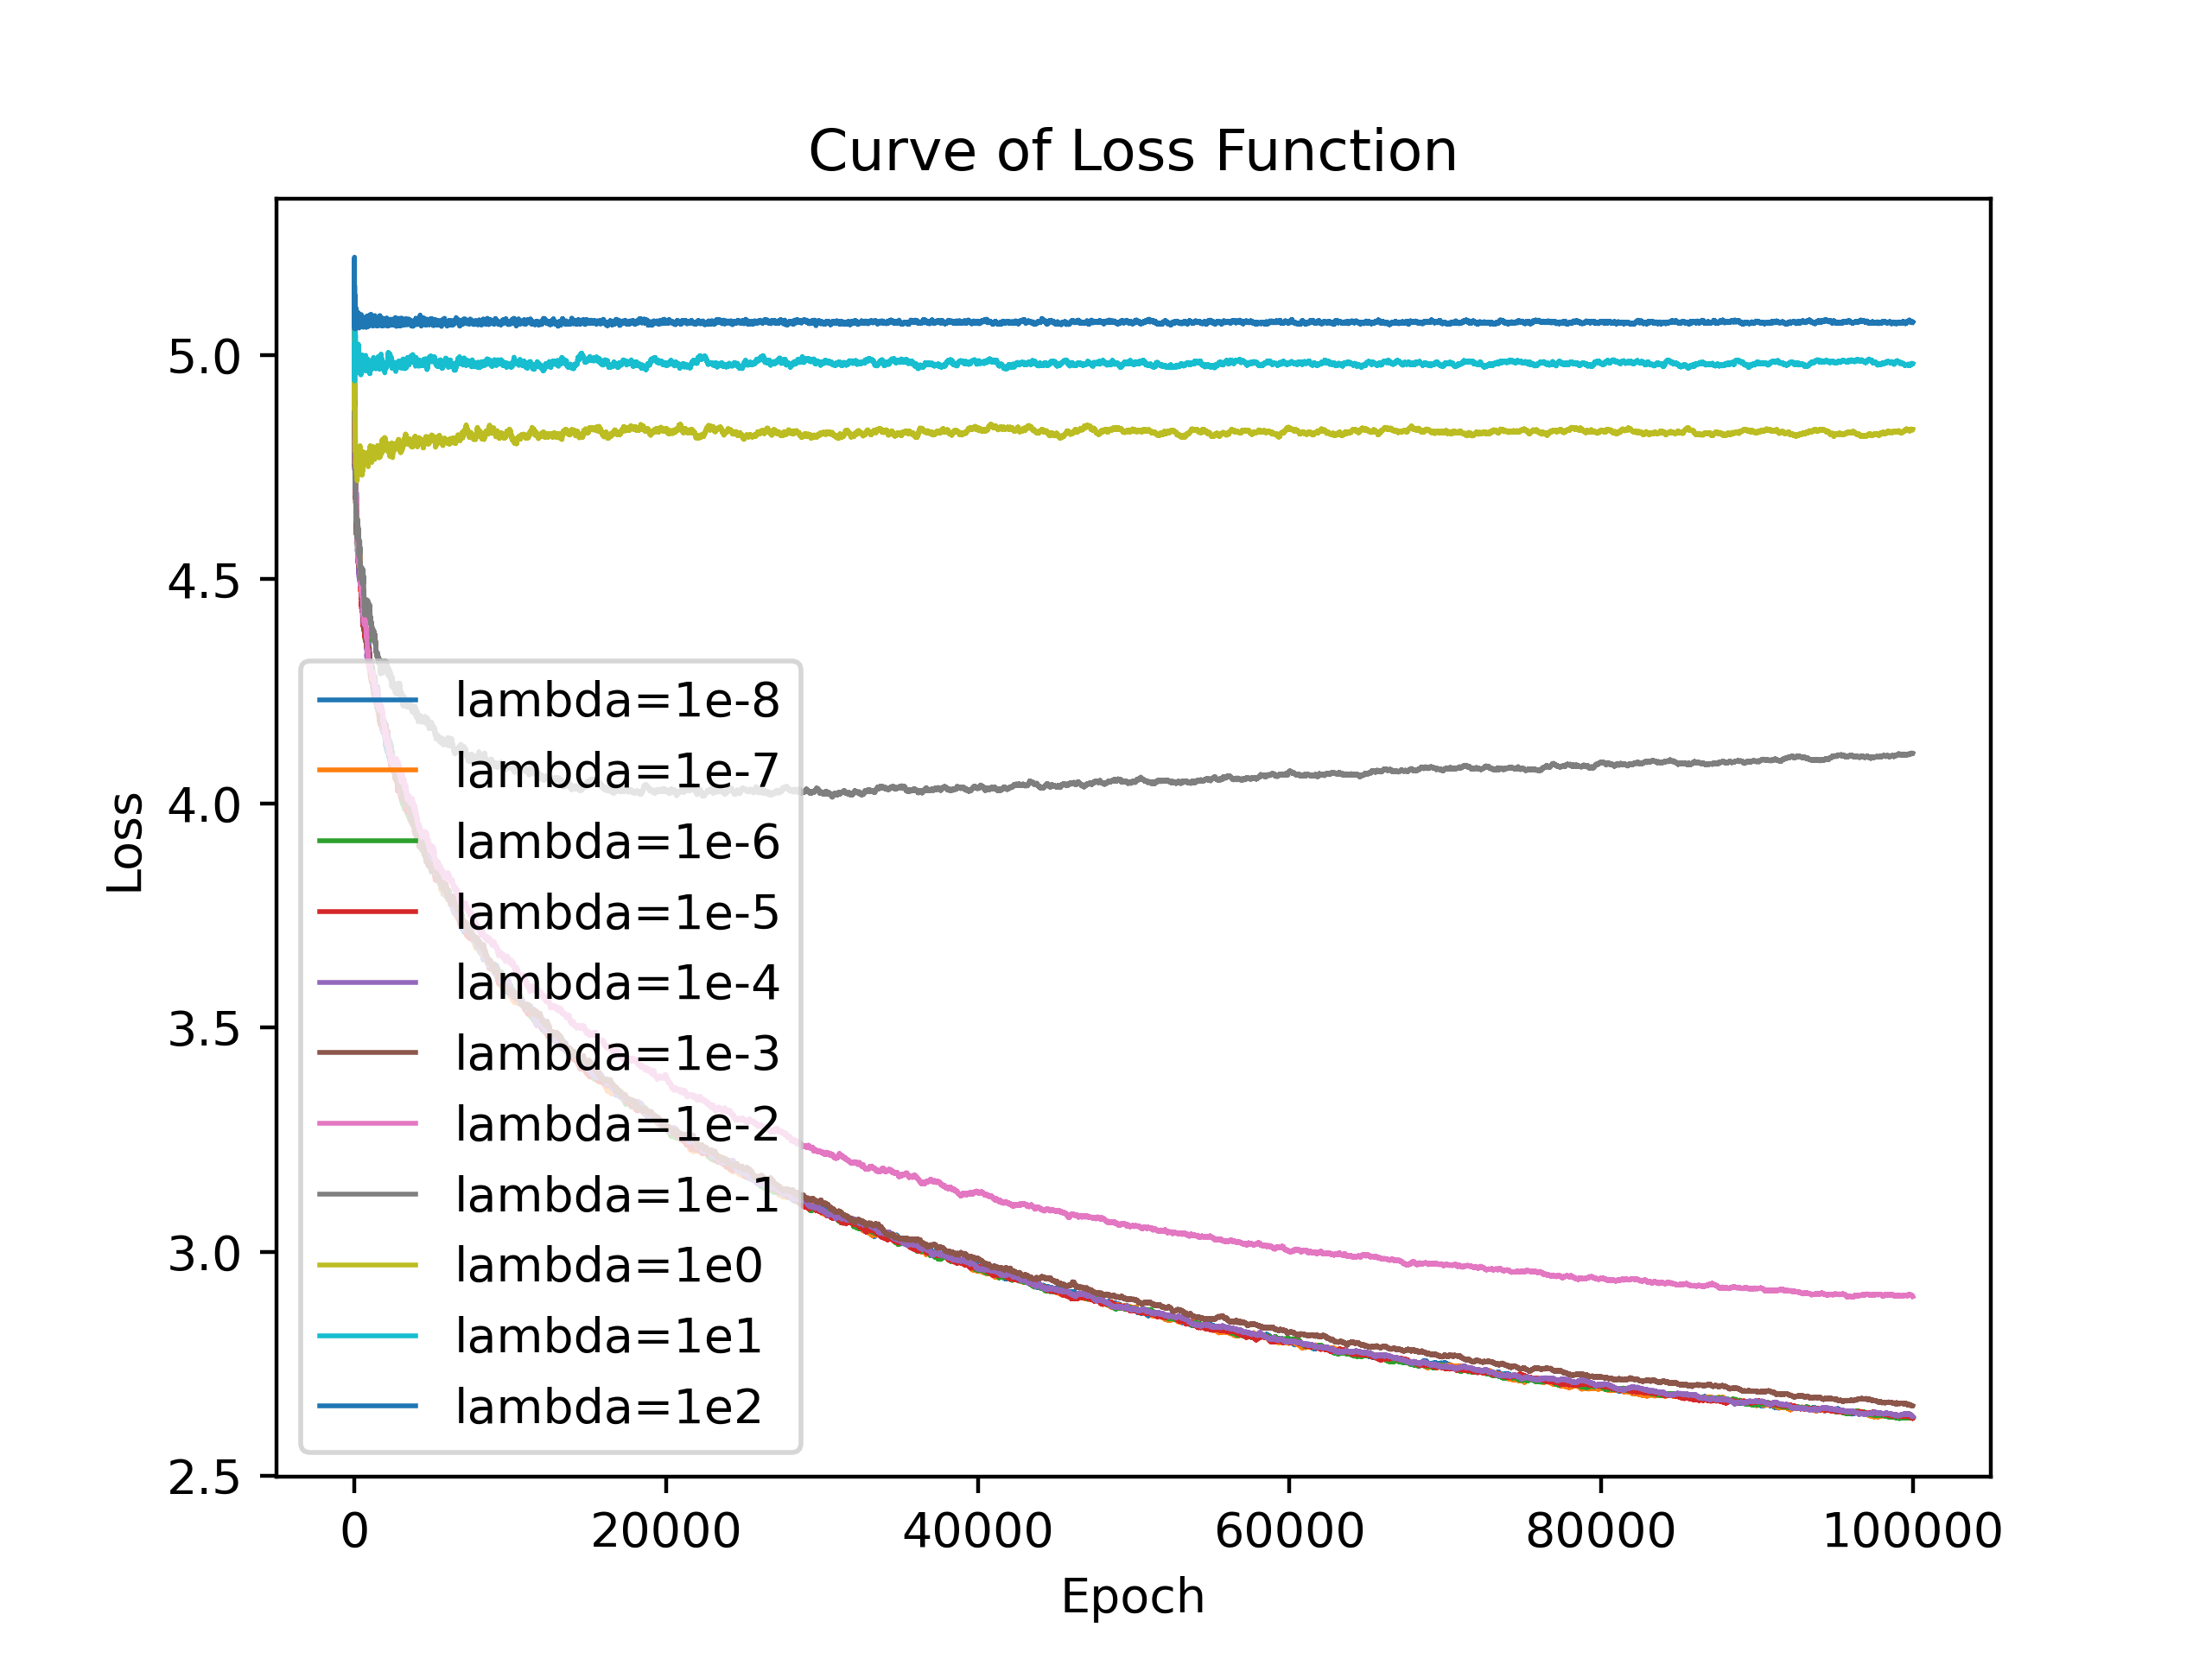
\includegraphics[width=0.84\textwidth]{./assets/SGD_lambda.png}
    \caption{不同正则化系数下验证集上的损失函数的变化曲线}
    \end{figure}

    从实验结果可以看出，当$\lambda \le 10^{-3}$时，模型误差较小。
    当$\lambda = 10^{-5}$时，模型效果最好，\textbf{在验证集上的均方误差为2.628}。

    \subsection{牛顿法}

    \subsubsection{目标函数的海森矩阵}

        根据题意，$J_{MSE}(\thetav) = \frac{1}{m} \Vert \Xm \thetav - \yv \Vert_2^2 + \lambda \thetav^T \thetav$，有：
        \begin{align*}
        \nabla J_{MSE}(\thetav) = \frac{2}{m} \Xm^T (\Xm \thetav - \yv) + 2 \lambda \thetav
        \end{align*}

        求微分：
        \begin{align*}
        d \nabla J_{MSE}(\thetav) = \frac{2}{m} \Xm^T \Xm d \thetav + 2 \lambda d \thetav
        = (\frac{2}{m} \Xm^T \Xm + 2 \lambda \imat{I})^T d \thetav
        \end{align*}

        因此目标函数的海森矩阵为：
        \begin{equation}\begin{aligned}
        \imat{H} = \nabla^2 J_{MSE} = \frac{2}{m} \Xm^T \Xm + 2 \lambda \imat{I}
        \end{aligned}\end{equation}

        任取非零向量$\xv \in \mathbb{R}^{d + 1}$，由于$\lambda > 0$，有：
        \begin{align*}
        \xv^T \imat{H} \xv
        &= \xv^T (\frac{2}{m} \Xm^T \Xm + 2 \lambda \imat{I}) \xv \\
        &= \frac{2}{m} (\xv^T \Xm^T \Xm \xv) + 2 \lambda \xv^T \xv \\
        &= \frac{2}{m} \Vert \Xm \xv \Vert_2^2 + 2 \lambda \Vert \xv \Vert_2^2 \\
        &\ge 2 \lambda \Vert \xv \Vert_2^2 > 0
        \end{align*}

        因此海森矩阵$\imat{H}$在$\lambda > 0$的情况下严格正定，因此一定非奇异。

    \subsubsection{基于牛顿法的梯度下降算法}

        略。

\section{支持向量机}

    \subsection{次梯度}

    \subsubsection{合页损失函数的次梯度}

        定义合页损失函数：
        \begin{equation}\begin{aligned}
        J(\omegav) = \max\{0, 1 - y \omegav^T \xv\}
        \end{aligned}\end{equation}

        合页损失函数的次梯度为：
        \begin{equation}\begin{aligned}
        \partial J(\omegav) =
        \begin{cases}
        \ivec{0}      & \text{if \quad} y \omegav^T \xv > 1 \\
        -y \ivec{x}^* & \text{if \quad} y \omegav^T \xv = 1 \\
        -y \xv        & \text{if \quad} y \omegav^T \xv < 1
        \end{cases}
        \end{aligned}\end{equation}

        其中$\xv^*$与$\xv^*$形状一致，且满足：对$\xv^*$的任意一个分量，其值都在0与$\xv$的对应分量之间。

    \subsubsection{次梯度与凸性的关系}

        对于一个处处存在次梯度的函数$f: \mathbb{R}^d \rightarrow \mathbb{R}$，反设$f$非凸，
        则存在$\xv_0 \text{、} \yv_0 \in \mathbb{R}^d$和$\lambda_0 \in (0, 1)$，使得：
        \begin{align*}
        \lambda_0 f(\xv_0) + (1 - \lambda_0) f(\yv_0) < f(\lambda_0 \xv_0 + (1 - \lambda_0) \yv_0)
        \end{align*}

        考虑$\lambda_0 \xv_0 + (1 - \lambda_0) \yv_0$处的次梯度，有以下不等式立：
        \begin{align*}
        f(\xv_0) &\ge f(\lambda_0 \xv_0 + (1 - \lambda_0) \yv_0) + (1 - \lambda_0) g^T (\xv_0 - \yv_0) \\
        f(\yv_0) &\ge f(\lambda_0 \xv_0 + (1 - \lambda_0) \yv_0) + \lambda_0 g^T (\yv_0 - \xv_0)
        \end{align*}

        将两不等式分别乘以$\lambda_0$和$1 - \lambda_0$，相加得：
        \begin{align*}
        \lambda_0 f(\xv_0) + (1 - \lambda_0) f(\yv_0) &\ge f(\lambda_0 \xv_0 + (1 - \lambda_0) \yv_0) \\
        &+ \lambda_0 (1 - \lambda_0) g^T (\xv_0 - \yv_0) \\
        &+ \lambda_0 (1 - \lambda_0) g^T (\yv_0 - \xv_0) \\
        &= f(\lambda_0 \xv_0 + (1 - \lambda_0) \yv_0)
        \end{align*}

        这与我们的反证假设相矛盾，因此$f$是凸函数。

    \subsection{感知机}

    \subsubsection{使用SSGD算法最小化感知机损失}

        考虑线性假设空间，预测值$\hat{y} = \omegav^T \xv$，定义感知损失为：
        \begin{align*}
        L(\omegav) = \max\{0, -y \omegav^T \xv\}
        \end{align*}

        参考(9)，取$L(\omegav)$的次梯度为：
        \begin{align*}
        \partial L(\omegav) =
        \begin{cases}
        \ivec{0}      & \text{if \quad} y \omegav^T \xv > 0 \\
        -y \xv        & \text{if \quad} y \omegav^T \xv \le 0
        \end{cases}
        \end{align*}

        在SSGD算法中，不妨令batch\_size为1，固定步长为1。
        设随机选取的训练集样本序号为$i$，权重更新公式可表示为：
        \begin{align*}
        \omegav{(k + 1)}
        &= \omegav^{(k)} - \partial L(\omegav) \\
        &=
        \begin{cases}
        \omegav^{(k)}             & \text{if \quad} y (\omegav^{(k)})^T \xv_i > 0 \\
        \omegav^{(k)} + y_i \xv_i & \text{if \quad} y (\omegav^{(k)})^T \xv_i \le 0
        \end{cases}
        \end{align*}

        而在感知机算法中，权重的更新方式是：
        遍历数据集，若$y (\omegav^{(k)})^T \xv_i \le 0$，
        则令$\omegav^{(k + 1)} = \omegav^{(k)} + y_i \xv_i$，
        否则令$\omegav^{(k + 1)} = \omegav^{(k)}$。

        同理于我们在2.4.2节中的证明，可以看出在期望意义下，两种算法的权重更新方式是完全一致的。

        我们再证明两种算法的停机条件一致。

        在SSGD算法中，损失函数$L(\omegav)$的最小值为0，
        在$\forall i \in \{1, 2, ...n\}$，均有$y (\omegav)^T \xv_i \le 0$时取到。
        这意味着：SSGD算法的停机条件是$y (\omegav)^T \xv_i \le 0$，$i = 1, 2, ..., n$，
        与感知机算法中的停机条件一致。

        综上，我们即证明了使用SSGD算法最小化感知机损失在一定条件下等价于感知机算法。

    \subsubsection{权重线性组合表示}

        由于$\omegav^{0} = \ivec{0} = \sum_{i = 1}^{n} 0 · \xv_i$，说明$\omegav^{0}$是输入数据的线性组合。
        而在感知机算法中，$\omegav$的更新量只可能是$y_j \xv_j = (\sum_{i = 1, i \ne j}^{n} 0 · \xv_i) + y_j · \xv_j$或$\ivec{0}$，也为输入数据的线性组合。
        因此，经过任意多次更新后，$\omegav$仍然是输入数据的线性组合。

    \subsection{软间隔支持向量机}

    软间隔支持向量机的Primal Problem为：
    \begin{equation}\begin{aligned}
    \min\limits_{\omegav \in \mathbb{R}^d, b \in \mathbb{R}, \xiv \in \mathbb{R}^m}& \frac{\lambda}{2} \Vert \omegav \Vert_2^2 + \frac{1}{m} \sum_{i = 1}^{m} \xi_i \\
    s.t.& \quad y_i (\omegav^T \xv_i + b) \ge 1 - \xi_i \\
        & \quad \xi_i \ge 0, i = 1, 2, ..., m
    \end{aligned}\end{equation}

    \subsubsection{拉格朗日方程}

        软间隔支持向量机Primal Problem的拉格朗日方程为：
        \begin{equation}\begin{aligned}
        &L(\omegav, b, \xiv, \alphav, \muv) = \\
        &\frac{\lambda}{2} \Vert \omegav \Vert_2^2 + \frac{1}{m} \sum_{i = 1}^{m} \xi_i + \sum_{i = 1}^{m} \alpha_i (1 - \xi_i - y_i (\omegav^T \xv_i + b)) - \sum_{i = 1}^{m} \mu_i \xi_i \\
        &\alpha_i \ge 0, \mu_i \ge 0, i = 1, 2, ..., m
        \end{aligned}\end{equation}

    \subsubsection{对偶形式}

        Primal Problem等价于求$\min\limits_{\omegav, b, \xiv} \max\limits_{\alphav, \muv} L(\omegav, b, \xiv, \alphav, \muv)$，我们有：
        \begin{equation}\begin{aligned}
        \min\limits_{\omegav, b, \xiv} \max\limits_{\alphav, \muv} L(\omegav, b, \xiv, \alphav, \muv) \ge \max\limits_{\alphav, \muv} \min\limits_{\omegav, b, \xiv} L(\omegav, b, \xiv, \alphav, \muv)
        \end{aligned}\end{equation}

        我们定义求解$\max\limits_{\alphav, \muv} \min\limits_{\omegav, b, \xiv} L(\omegav, b, \xiv, \alphav, \muv)$为软间隔支持向量机的Dual Problem。
        由不等式(12)，Dual Problem的解是Primal Problem的一个近似解。

        求解驻点条件：
        \begin{align*}
        \frac{\partial L}{\partial \omegav} &= \lambda \omegav - \sum_{i = 1}^{m} \alpha_i y_i \xv_i = \ivec{0} \\
        \frac{\partial L}{\partial b} &= \sum_{i = 1}^{m} (- \alpha_i y_i) = 0 \\
        \frac{\partial L}{\partial \xi_i} &= \frac{1}{m} - \alpha_i - \mu_i = 0
        \end{align*}

        在Dual Problem的解中，应满足驻点条件，有：
        \begin{align*}
        \sum_{i = 1}^{m} \alpha_i y_i \xv_i &= \lambda \omegav \\
        \sum_{i = 1}^{m} \alpha_i y_i &= 0 \\
        \alpha_i + \mu_i &= \frac{1}{m}
        \end{align*}

        代入Dual Problem形式中：
        \begin{align*}
        \max\limits_{\alphav, \muv} \min\limits_{\omegav, b, \xiv} L(\omegav, b, \xiv, \alphav, \muv)
        &= \max\limits_{\alphav, \muv}\{\frac{\lambda}{2} \Vert \omegav \Vert_2^2 + \sum_{i = 1}^{m} \alpha_i - \sum_{i = 1}^{m} \alpha_i y_i \omegav^T \xv_i\} \\
        &= \max\limits_{\alphav}\{\sum_{i = 1}^{m} \alpha_i - \frac{1}{2 \lambda} \Vert \sum_{i = 1}^{m} \alpha_i y_i \xv_i \Vert_2^2\} \\
        s.t.& \quad \sum_{i = 1}^{m} \alpha_i y_i = 0, 0 \le \alpha_i \le \frac{1}{m}, i = 1, 2, ..., m
        \end{align*}

        于是，软间隔支持向量机的对偶形式即为：
        \begin{align*}
        \max\limits_{\alphav}\{\sum_{i = 1}^{m} \alpha_i - \frac{1}{2 \lambda} \Vert \sum_{i = 1}^{m} \alpha_i y_i \xv_i \Vert_2^2\} \\
        s.t. \quad \sum_{i = 1}^{m} \alpha_i y_i = 0, 0 \le \alpha_i \le \frac{1}{m}, i = 1, 2, ..., m
        \end{align*}

    \subsubsection{使用核函数的软间隔支持向量机}

        在引入非线性映射$\Phi$和对应的核函数$k(·,·)$后，软间隔支持向量机的Primal Problem变为：
        \begin{equation}\begin{aligned}
        \min\limits_{\omegav \in \mathbb{R}^d, b \in \mathbb{R}, \xiv \in \mathbb{R}^m}& \frac{\lambda}{2} \Vert \omegav \Vert_2^2 + \frac{1}{m} \sum_{i = 1}^{m} \xi_i \\
        s.t.& \quad y_i (\omegav^T \Phi(\xv_i) + b) \ge 1 - \xi_i \\
            & \quad \xi_i \ge 0, i = 1, 2, ..., m
        \end{aligned}\end{equation}

        由Representer Theorem，最优的权重$\omegav$必然是样本输入的的线性组合，因此不妨设：$\omegav = \sum_{i = 1}^{m} \gamma_i \Phi(\xv_i)$，
        代入Primal Problem中可得：
        \begin{equation}\begin{aligned}
        \min\limits_{\omegav \in \mathbb{R}^d, b \in \mathbb{R}, \xiv \in \mathbb{R}^m}& \frac{\lambda}{2} (\sum_{i = 1}^{m} \sum_{j = 1}^{m} \gamma_i \gamma_j k(\xv_i, \xv_j)) + \frac{1}{m} \sum_{i = 1}^{m} \xi_i \\
        s.t.& \quad y_i (\sum_{j = 1}^{m} \gamma_j k(\xv_i, \xv_j) \Phi(\xv_i) + b) \ge 1 - \xi_i \\
            & \quad \xi_i \ge 0, i = 1, 2, ..., m
        \end{aligned}\end{equation}

        类似地，使用核函数后，Dual Problem变为：
        \begin{equation}\begin{aligned}
        \max\limits_{\alphav}\{\sum_{i = 1}^{m} \alpha_i - \frac{1}{2 \lambda} \sum_{i = 1}^{m} \sum_{j = 1}^{m} \alpha_i \alpha_j y_i y_j k(\xv_i, \xv_j)\} \\
        s.t. \quad \sum_{i = 1}^{m} \alpha_i y_i = 0, 0 \le \alpha_i \le \frac{1}{m}, i = 1, 2, ..., m
        \end{aligned}\end{equation}

    \subsubsection{使用次梯度下降算法求解SVM}

        考虑SVM的损失函数为：
        \begin{equation}\begin{aligned}
        J_i(\omegav, b) = \frac{\lambda}{2} \Vert \omegav \Vert_2^2 + \max\{0, 1 - y_i (\omegav^T \xv_i + b)\}
        \end{aligned}\end{equation}

        记$l_i(\omegav, b) = \max\{0, 1 - y_i (\omegav^T \xv_i + b)\}$，则(16)式又可表示为：
        \begin{align*}
        J_i(\omegav, b) = \frac{\lambda}{2} \Vert \omegav \Vert_2^2 + l_i(\omegav, b)
        \end{align*}

        在$J_i$中，$\frac{\lambda}{2} \Vert \omegav \Vert_2^2$在定义域上均连续可导，有：
        $\frac{\partial (\frac{\lambda}{2} \Vert \omegav \Vert_2^2)}{\partial \omegav} = \lambda \omegav$，
        $\frac{\partial (\frac{\lambda}{2} \Vert \omegav \Vert_2^2)}{\partial b} = \ivec{0}$。

        因此，我们只需验证
        $\partial J_i \big|_{\omegav} = \begin{cases}
        -y_i \xv_i & \text{if \quad} y_i (\omegav^T \xv_i + b) < 1 \\
        \ivec{0}   & \text{if \quad} y_i (\omegav^T \xv_i + b) \ge 1
        \end{cases}$是$l_i$关于$\omegav$的次梯度，验证
        $\partial J_i \big|_b = \begin{cases}
        -y_i & \text{if \quad} y_i (\omegav^T \xv_i + b) < 1 \\
        0    & \text{if \quad} y_i (\omegav^T \xv_i + b) \ge 1
        \end{cases}$是$l_i$关于$b$的次梯度即可。

        对于前者，考虑任意和$\omegav$形状相同的$\omegav_*$，记：
        \begin{align*}
        \Delta_{\omegav}(\omegav_*) = l_i(\omegav_*, b) - l_i(\omegav, b) - (\partial J_i \big|_{\omegav}(\omegav))^T (\omegav_* - \omegav)
        \end{align*}

        我们下面证明$\Delta_{\omegav}(\omegav_*) \ge 0$恒成立：

        若$y_i(\omegav^T \xv_i + b) \ge 1$，则：
        \begin{align*}
        \Delta_{\omegav}(\omegav_*) = l_i(\omegav_*, b) \ge 0
        \end{align*}

        若$y_i(\omegav^T \xv_i + b) < 1$，则：
        \begin{align*}
        \Delta_{\omegav}(\omegav_*)
        &= l_i(\omegav_*, b) - (1 - y_i (\omegav^T \xv_i + b)) + y_i \xv_i^T (\omegav_* - \omegav) \\
        &= \max\{0, 1 - y_i (\omegav_*^T \xv_i + b)\} - (1 - y_i (\omegav_*^T \xv_i + b)) \\
        &\ge 0
        \end{align*}

        对于后者，考虑任意$b_* \in \mathbb{R}$，记：
        \begin{align*}
        \Delta_{b}(b_*) = l_i(\omegav, b_*) - l_i(\omegav, b) - \partial J_i \big|_{b}(b) (b_* - b)
        \end{align*}

        我们下面证明$\Delta_{b}(b_*) \ge 0$恒成立：

        若$y_i(\omegav^T \xv_i + b) \ge 1$，则：
        \begin{align*}
        \Delta_{b}(b_*) = l_i(\omegav_*, b) \ge 0
        \end{align*}

        若$y_i(\omegav^T \xv_i + b) < 1$，则：
        \begin{align*}
        \Delta_{b}(b_*)
        &= l_i(\omegav, b_*) - (1 - y_i (\omegav \xv_i + b)) + y_i (b_* - b) \\
        &= \max\{0, 1 - y_i (\omegav^T \xv_i + b_*)\} - (1 - y_i (\omegav^T \xv_i + b_*)) \\
        &\ge 0
        \end{align*}

        综上，我们即证明了题目中给出的SVM的损失函数次梯度的正确性。

    \subsubsection{使用SSGD算法训练SVM的伪代码}

        以下是使用SSGD算法训练SVM的伪代码，这里不妨考虑batch\_size为1的情况。

        \begin{algorithm}[htbp]
        \caption{Training SVM with SSGD}
        \begin{algorithmic}[1]
            \Require $(\xv_1, y_1), (\xv_2, y_2), ..., (\xv_m, y_m) \in \mathbb{R}^d \times \{1, -1\}$
            \Ensure $\omegav \in \mathbb{R}^d, b \in \mathbb{R}$ which minimize loss function $J$
            \State $\omegav^{(0)} \gets \ivec{0}$
            \State $b^{(0)} \gets 0$
            \For{$epoch = 1, 2, ...,T$} \Comment{$T$为迭代次数}
                \State choose $(\xv_i, y_i)$ from input randomly
                \State compute subgradient $\delta_{\omega} \gets \partial J_i \big|_{\omegav}(\omegav^{(epoch - 1)}), \delta_{b} \gets \partial J_i \big|_{b}(b^{(epoch - 1)})$
                \State update $\omegav^{(epoch)} \gets (\omegav^{(epoch - 1)} - \eta \delta_{\omega})$ \Comment{$\eta$为学习率}
                \State update $b^{(epoch)} \gets (b^{(epoch - 1)} - \eta \delta_{b})$
            \EndFor
            \State \Return $\omegav^{(T)}, b^{(T)}$
        \end{algorithmic}
        \end{algorithm}

    \subsubsection{带L2正则项的软间隔支持向量机}

        对于带L2正则项的软间隔支持向量机，其Primal Problem为：
        \begin{equation}\begin{aligned}
        \min\limits_{\omegav \in \mathbb{R}^d, b \in \mathbb{R}, \xiv \in \mathbb{R}^m}& \frac{\lambda}{2} \Vert \omegav \Vert_2^2 + \frac{1}{m} \sum_{i = 1}^{m} \xi_i^2 \\
        s.t.& \quad y_i (\omegav^T \xv_i + b) \ge 1 - \xi_i, i = 1, 2, ..., m
        \end{aligned}\end{equation}

        设Primal Problem中优化函数的最小值为$m_0$，我们证明，一定存在$\xiv$，满足$\xi_i \ge 0$，$i = 1, 2, ..., m$，
        使得优化函数可以取到最小值$m_0$。

        任取一个使优化函数取到最小值$m_0$的解$(\omegav^*, b^*, \xiv^*)$。
        我们取$\xiv^{+*}$，满足$\xi_i^{+*} = \vert \xi_i^* \vert \ge 0$，$i = 1, 2, ..., m$。
        显然有$\frac{1}{m} \sum_{i = 1}^{m} \xi_i^{*2} = \frac{1}{m} \sum_{i = 1}^{m} \xi_i^{+*2}$成立。

        而对于任意的$i=1, 2, ..., m$，注意到：$y_i (\omegav^{*T} \xv_i^* + b^*) \ge 1 - \xi_i^* \ge 1 - \xi^{+*}$。

        因此，$(\omegav^*, b^*, \xiv^{+*})$也是使优化函数取到最小值$m_0$的一组解，且$\xi_i^{+*} \ge 0$，$i = 1, 2, ..., m$。

        这也解释了为什么我们可以省略$\xi_i \ge 0$这一约束。

    \subsubsection{带L2正则项的软间隔支持向量机的拉格朗日方程与对偶形式}

        带L2正则项的软间隔支持向量机Primal Problem的拉格朗日方程为：
        \begin{equation}\begin{aligned}
        &L(\omegav, b, \xiv, \alphav) = \\
        &\frac{\lambda}{2} \Vert \omegav \Vert_2^2 + \frac{1}{m} \sum_{i = 1}^{m} \xi_i^2 + \sum_{i = 1}^{m} \alpha_i (1 - \xi_i - y_i (\omegav^T \xv_i + b)) \\
        &\alpha_i \ge 0, i = 1, 2, ..., m
        \end{aligned}\end{equation}

        求解驻点条件：
        \begin{align*}
        \frac{\partial L}{\partial \omegav} &= \lambda \omegav - \sum_{i = 1}^{m} \alpha_i y_i \xv_i = \ivec{0} \\
        \frac{\partial L}{\partial b} &= \sum_{i = 1}^{m} (- \alpha_i y_i) = 0 \\
        \frac{\partial L}{\partial \xi_i} &= \frac{2}{m} \xi_i - \alpha_i = 0
        \end{align*}

        在Dual Problem的解中，应满足驻点条件，有：
        \begin{align*}
        \sum_{i = 1}^{m} \alpha_i y_i \xv_i &= \lambda \omegav \\
        \sum_{i = 1}^{m} \alpha_i y_i &= 0 \\
        \frac{m}{2} \alpha_i &= \xi_i
        \end{align*}

        代入Dual Problem形式中：
        \begin{align*}
        \max\limits_{\alphav} \min\limits_{\omegav, b, \xiv} L(\omegav, b, \xiv, \alphav)
        &= \max\limits_{\alphav}\{\frac{\lambda}{2} \Vert \omegav \Vert_2^2 + \sum_{i = 1}^{m} (- \frac{m}{4}\alpha_i^2 + \alpha_i) - \sum_{i = 1}^{m} \alpha_i y_i \omegav^T \xv_i\} \\
        &= \max\limits_{\alphav}\{\sum_{i = 1}^{m} (- \frac{m}{4}\alpha_i^2 + \alpha_i) - \frac{1}{2 \lambda} \Vert \sum_{i = 1}^{m} \alpha_i y_i \xv_i \Vert_2^2\} \\
        s.t.& \quad \sum_{i = 1}^{m} \alpha_i y_i = 0, \alpha_i \ge 0, i = 1, 2, ..., m
        \end{align*}

        于是，带L2正则项的软间隔支持向量机的对偶形式即为：
        \begin{align*}
        \max\limits_{\alphav}\{\sum_{i = 1}^{m} (- \frac{m}{4}\alpha_i^2 + \alpha_i) - \frac{1}{2 \lambda} \Vert \sum_{i = 1}^{m} \alpha_i y_i \xv_i \Vert_2^2\} \\
        s.t. \quad \sum_{i = 1}^{m} \alpha_i y_i = 0, \alpha_i \ge 0, i = 1, 2, ..., m
        \end{align*}

    \subsection{情绪检测}

    \subsubsection{使用SSGD算法训练线性SVM模型}

        已实现，参见./SVM/startcode.py中的linear\_svm\_subgrad\_descent函数。

    \subsubsection{超参数调整}

        调整超参数，我们希望训练得到的线性SVM模型能获得更好的性能。
        我们将通过四次单变量实验，分别对步长、正则化系数、批大小和迭代次数进行调整。
        在不同的超参数下，我们记录了模型在训练集和验证集上的准确率变化情况，如表2、表3、表4、表5所示。

        \begin{table}[htbp]
        \caption{调整步长，模型在训练集和验证集上的准确率变化情况}
        \centering
        \begin{tabular}{cccccc}
            \toprule
            步长           & 正则化系数 & 批大小 & 迭代次数 & Acc (train) & Acc (valid)        \\
            \midrule
            0.005          &  0.0001   &   1    &  60000  &  0.785890   &  0.749819          \\
            0.010          &  0.0001   &   1    &  60000  &  0.883436   &  0.827910          \\
            \textbf{0.050} &  0.0001   &   1    &  60000  &  0.953988   &  \textbf{0.867679} \\
            0.100          &  0.0001   &   1    &  60000  &  0.962883   &  0.841649
        \end{tabular}
        \end{table}

        \begin{table}[htbp]
        \caption{调整正则化系数，模型在训练集和验证集上的准确率变化情况}
        \centering
        \begin{tabular}{cccccc}
            \toprule
            步长  & 正则化系数         & 批大小 & 迭代次数 & Acc (train) & Acc (valid)        \\
            \midrule
            0.050 &  0.00005          &   1    &  60000  &  0.957055   &  0.858279          \\
            0.050 &  \textbf{0.00010} &   1    &  60000  &  0.953988   &  \textbf{0.867679} \\
            0.050 &  0.00020          &   1    &  60000  &  0.950307   &  0.866233          \\
            0.050 &  0.00050          &   1    &  60000  &  0.942331   &  0.857556
        \end{tabular}
        \end{table}

        \begin{table}[htbp]
        \caption{调整批大小，模型在训练集和验证集上的准确率变化情况}
        \centering
        \begin{tabular}{cccccc}
            \toprule
            步长  & 正则化系数 & 批大小      & 迭代次数 & Acc (train) & Acc (valid)        \\
            \midrule
            0.050 &  0.00010  &  \textbf{1} &  60000  &  0.953988   &  \textbf{0.867679} \\
            0.050 &  0.00010  &  4          &  60000  &  0.957362   &  0.863341          \\
            0.050 &  0.00010  &  16         &  60000  &  0.958589   &  0.864787          \\
            0.050 &  0.00010  &  64         &  60000  &  0.956748   &  0.862617
        \end{tabular}
        \end{table}

        \begin{table}[htbp]
        \caption{调整迭代次数，模型在训练集和验证集上的准确率变化情况}
        \centering
        \begin{tabular}{cccccc}
            \toprule
            步长  & 正则化系数 & 批大小 & 迭代次数        & Acc (train) & Acc (valid)        \\
            \midrule
            0.050 &  0.00010  &   1    & 10000          &  0.876994   &  0.814172          \\
            0.050 &  0.00010  &   1    & 30000          &  0.935890   &  0.859725          \\
            0.050 &  0.00010  &   1    & \textbf{60000} &  0.953988   &  \textbf{0.867679} \\
            0.050 &  0.00010  &   1    & 100000         &  0.967791   &  0.866956
        \end{tabular}
        \end{table}

        综上，我们取步长为0.05，正则化系数为0.0001，批大小为1，迭代次数为60000次时，模型的性能较好，
        \textbf{在训练集上的准确率为95.40\%}，\textbf{在验证集上的准确率为86.77\%}。

    \subsubsection{收敛更快速的优化算法}

        我们首先估测题述算法的收敛速度。

        设优化目标函数为$f(\omegav)$，它是$\lambda$-强凸的。由$\lambda$-强凸性的定义，有以下不等式成立：
        \begin{align*}
        f(\omegav^{(t)}) - f(\omegav^*) \le \ivec{\nu}_t^T (\omegav^{(t)} - \omegav^*) - \frac{\lambda}{2} \Vert \omegav^{(t)} - \omegav^* \Vert_2^2
        \end{align*}

        根据题述算法的迭代过程，我们有$\ivec{\nu}_t = \lambda t (\omegav^{(t)} - \omegav^{(t + 1)})$，代入上式：
        \begin{align*}
        &f(\omegav^{(t)}) - f(\omegav^*) \\
        \le& \lambda t (\omegav^{(t)} - \omegav^{(t + 1)})^T (\omegav^{(t)} - \omegav^*) - \frac{\lambda}{2} \Vert \omegav^{(t)} - \omegav^* \Vert_2^2 \\
        =  & \frac{\lambda t}{2} (\Vert \omegav^{(t)} - \omegav^* \Vert_2^2 - \Vert \omegav^{(t + 1)} - \omegav^* \Vert_2^2 + \Vert \omegav^{(t + 1)} - \omegav^{(t)} \Vert_2^2) - \frac{\lambda}{2} \Vert \omegav^{(t)} - \omegav^* \Vert_2^2\\
        \le& \frac{\lambda }{2} ((t - 1) \Vert \omegav^{(t)} -  \omegav^* \Vert_2^2 - t \Vert \omegav^{(t + 1)} - \omegav^* \Vert_2^2) + \frac{\lambda t}{2} \Vert \omegav^{(t + 1)} - \omegav^{(t)} \Vert_2^2
        \end{align*}

        对$t$求和：
        \begin{align*}
        \sum_{t = 1}^{T} (f(\omegav^{(t)}) - f(\omegav^*))
        \le& - \frac{\lambda T}{2} \Vert \omegav^{(T + 1)} - \omegav^* \Vert_2^2 + \frac{\lambda}{2} \sum_{t = 1}^{T} t \Vert \omegav^{(t + 1)} - \omegav^{(t)} \Vert_2^2 \\
        \le& \frac{\lambda}{2} \sum_{t = 1}^{T} t (\frac{\ivec{\nu}_t}{\lambda t})^2 = \frac{1}{2 \lambda} \sum_{t = 1}^{T} \frac{\ivec{\nu}_t^2}{t}
        \end{align*}

        在强凸函数中，次梯度$\ivec{\nu}$有界，因此存在常数$C > 0$，使得$\ivec{\nu}^2 < C$恒成立。于是：
        \begin{align*}
        \sum_{t = 1}^{T} (f(\omegav^{(t)}) - f(\omegav^*)) \le \frac{C}{2 \lambda} \sum_{t = 1}^{T} \frac{1}{t} \le \frac{C}{2 \lambda} (1 + \log(T))
        \end{align*}

        于是：
        \begin{equation}\begin{aligned}
        \frac{1}{T} \sum_{t = 1}^{T} (f(\omegav^{(t)}) - f(\omegav^*)) \le \frac{C}{2 \lambda} \frac{1 + \log(T)}{T}
        \end{aligned}\end{equation}

        这即证明了题述算法的收敛速度是$O(\frac{\log(T)}{T})$，小于一般的收敛速度$O(\frac{1}{\sqrt{T}})$。

        在./SVM/startcode.py中的linear\_svm\_subgrad\_descent\_lambda函数有该算法的实现。
        除题述算法外，我们还实现了取权重平均为输出权重值的算法。

        我们记录了两种算法在训练过程中的损失函数值的变化情况如图8所示。
        其中在普通算法中，我们考虑了步长为0.05和0.001两种情形。
        为了消去随机下降中的振荡现象，我们总是记录每10个epoch中最小一个的损失函数值。

        \begin{figure}[htbp]
        \centering
        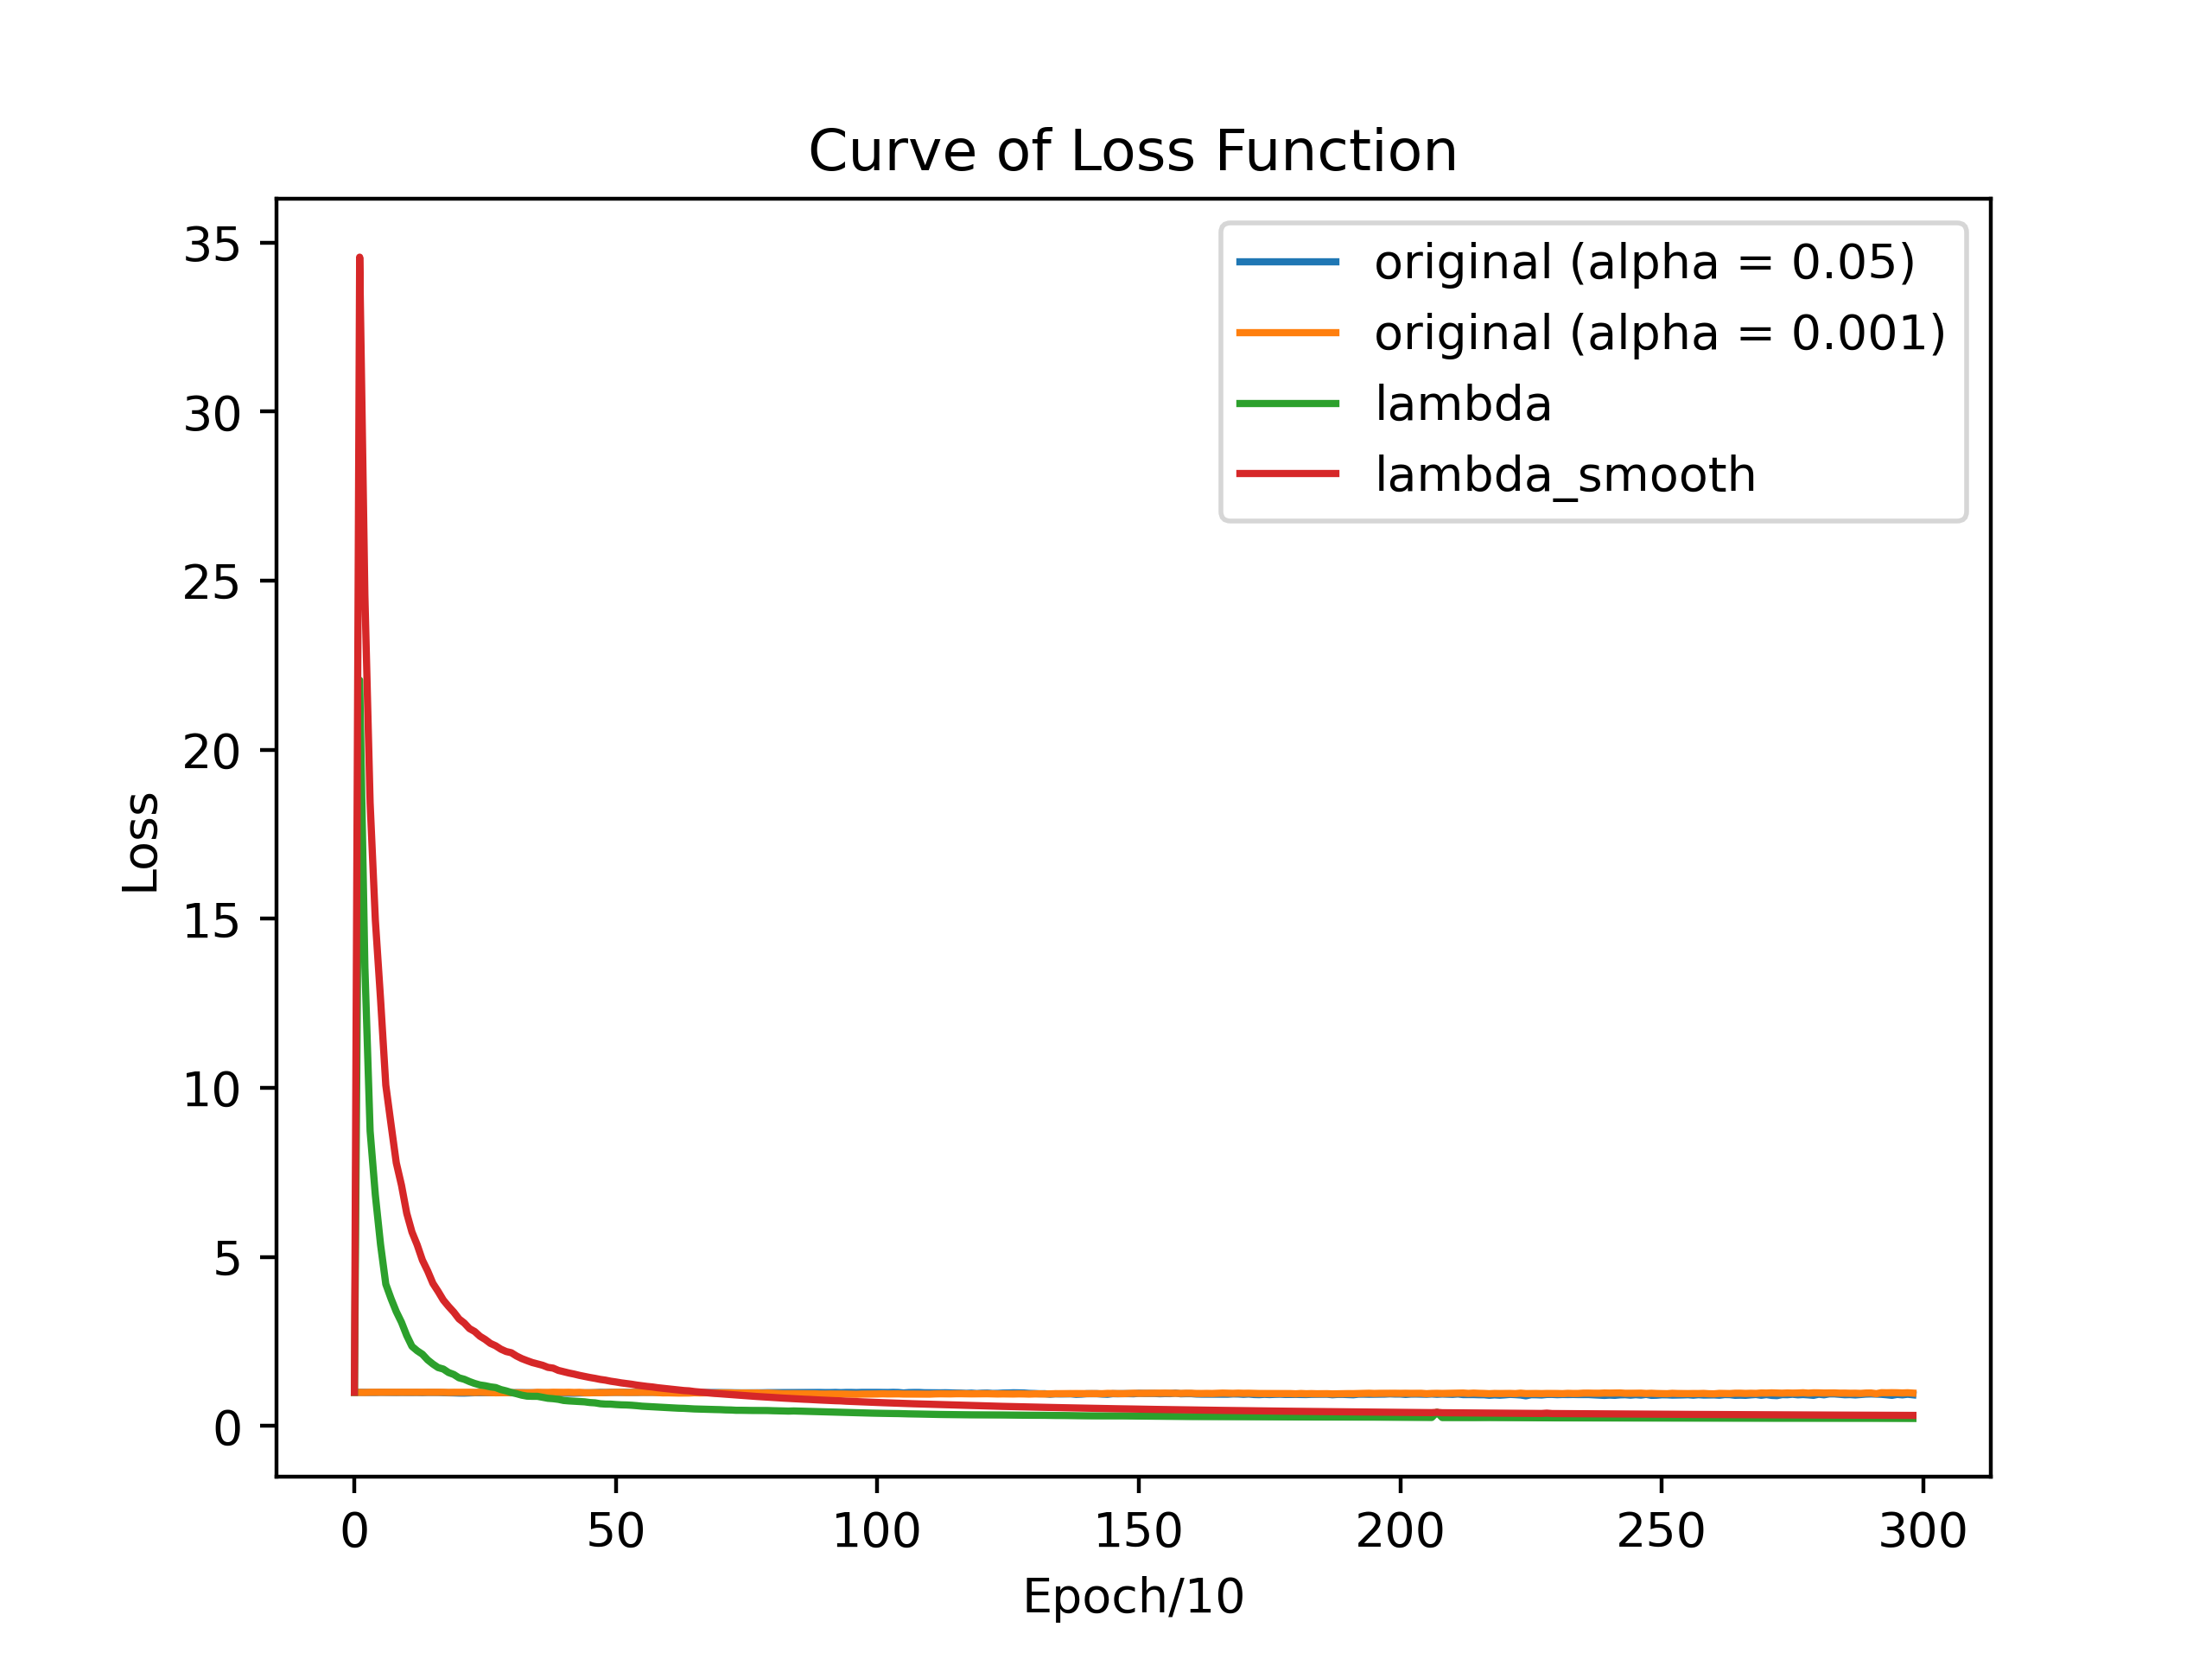
\includegraphics[width=0.84\textwidth]{./assets/SVM_lambda.png}
        \caption{不同算法下，SVM模型在训练过程中的损失函数的变化曲线}
        \end{figure}

        可以看出，虽然强凸函数的优化算法在训练初期不太平稳，但是在约300次迭代后，
        其收敛情况已经趋于平稳，体现出超越一般算法的优化效率，
        最终还能使模型收敛到损失函数值更低的位置。
        而在强凸函数的优化算法的两种实现上，我们发现采用直接输出权重的方式效果更好。

    \subsubsection{基于核函数的SVM}

        在./SVM/startcode.py中的kernel\_svm\_subgrad\_descent函数中，我们实现了基于径向核函数的SVM模型。

        我们首先参考课件中的伪代码实现了第一个版本的算法。
        但是在调参过程中，我们发现算法难以收敛，推测问题出在步长策略上，基于径向核函数的SVM模型可能不能在固定步长下训练。

        因此，我们参考了《Understanding Machine Learning: From Theory to Algorithms》一书中16.3节的有关内容，
        实现了第二个版本的算法，效果较好。该算法的伪代码如图9所示。

        \begin{figure}[htbp]
        \centering
        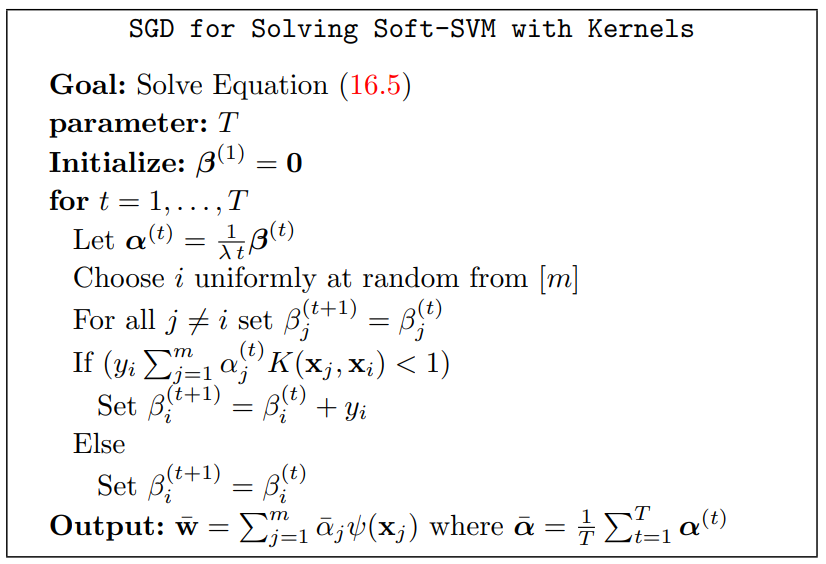
\includegraphics[width=0.84\textwidth]{./assets/K_SVM.png}
        \caption{改进的基于径向核函数的SVM模型的优化算法}
        \end{figure}

        表6、表7、表8是调参的实验结果，我们主要调整了正则化系数、迭代次数和批大小三个超参数。

        \begin{table}[htbp]
        \caption{调整批大小，模型在训练集和验证集上的准确率变化情况}
        \centering
        \begin{tabular}{ccccc}
            \toprule
            正则化系数 & 批大小       & 迭代次数 & Acc (train) & Acc (valid)       \\
            \midrule
            0.001     &  1           &  1000   &  0.818405   &  0.746204          \\
            0.001     &  4           &  1000   &  0.882209   &  0.809111          \\
            0.001     &  16          &  1000   &  0.920552   &  0.836587          \\
            0.001     &  \textbf{64} &  1000   &  0.939877   &  \textbf{0.852495}
        \end{tabular}
        \end{table}

        \begin{table}[htbp]
        \caption{调整正则化系数，模型在训练集和验证集上的准确率变化情况}
        \centering
        \begin{tabular}{ccccc}
            \toprule
            正则化系数       & 批大小 & 迭代次数 & Acc (train) & Acc (valid)       \\
            \midrule
            0.0001          &   64   &  1000   &  0.945092   &  0.845987          \\
            0.0005          &   64   &  1000   &  0.938037   &  0.840202          \\
            \textbf{0.0010} &   64   &  1000   &  0.939877   &  \textbf{0.852495} \\
            0.0050          &   64   &  1000   &  0.927607   &  0.845987
        \end{tabular}
        \end{table}

        \begin{table}[htbp]
        \caption{调整迭代次数，模型在训练集和验证集上的准确率变化情况}
        \centering
        \begin{tabular}{cccccc}
            \toprule
            正则化系数 & 批大小 & 迭代次数        & Acc (train) & Acc (valid)       \\
            \midrule
            0.001     &  64    &  500           &  0.899387   &  0.825741          \\
            0.001     &  64    &  1000          &  0.939877   &  0.852495          \\
            0.001     &  64    &  2000          &  0.976074   &  0.854664          \\
            0.001     &  64    &  \textbf{5000} &  0.995399   &  \textbf{0.869848}
        \end{tabular}
        \end{table}

        综上，我们取正则化系数为0.001，批大小为64，迭代次数为5000次时，模型的性能较好，
        \textbf{在训练集上的准确率为99.54\%}，\textbf{在验证集上的准确率为86.98\%}。

        我们发现，相比于一般的SVM模型，在引入核函数后，模型的在训练集上的准确率明显提升（95.40\% -> 99.54\%），说明核函数提高了模型的拟合能力。
        在验证集上，引入核函数后模型的准确率有一定的提升（86.77\% -> 86.98\%），但是提升幅度并不明显。我们认为可能的原因有两点：

        1. 我们输入的词向量空间维度很高，导致词向量在空间中的分布非常稀疏。
        因此，线性超平面的分类效果和采用基函数变换后的超平面分类效果差距并不明显。

        2. 注意到在引入核函数后，模型在训练集上的准确率已经接近100\%，这说明模型此时已经几乎将训练集中的数据完全分类。
        在不引入更多的先验知识的情况下，SVM模型的性能将很难再进一步提高了。

    \subsubsection{最终模型的性能总结}

        使用基于径向核函数的SVM模型，取正则化系数为0.001，批大小为64，迭代次数为10000次。
        我们以此作为我们的最终模型。

        \textbf{在验证集上，其混淆矩阵为$\begin{bmatrix} 609 & 92 \\ 98 & 584 \end{bmatrix}$；
        准确率为86.51\%，精确率为86.88\%，召回率为86.14\%；F1-Score等于0.8651。}

\end{document}
